% =============================================================================
% SW705 - Taller de Ingenieria de Software I (UNI - FIIS)
% Guia practica - Semana 6: Diseno de datos y prototipo UX/UI
% Entregable 4 (Classroom) = Avance 3 del proyecto integrador
% Grupo A - Sistema SIRA - Clinica San Rafael S.A.C.
%
% Compilar con pdfLaTeX (Overleaf: Menu > Compiler > pdfLaTeX).
% Las notas para el equipo van como comentarios (%) y no salen en el PDF.
% =============================================================================
\documentclass[11pt,a4paper]{article}

% ---------------------------------------------------------------- Idioma
\usepackage[utf8]{inputenc}
\usepackage[T1]{fontenc}
\usepackage[spanish,es-tabla,es-noshorthands]{babel}
\usepackage{lmodern}
\usepackage{amssymb}

% ---------------------------------------------------------------- Pagina
\usepackage[margin=2.2cm,headheight=15pt]{geometry}
\usepackage{fancyhdr}
\usepackage{titlesec}
\usepackage{titletoc}

% ---------------------------------------------------------------- Tablas y figuras
\usepackage[table]{xcolor}
\usepackage{array}
\usepackage{tabularx}
\usepackage{xltabular}
\usepackage{graphicx}
\graphicspath{{./}{figuras/}{../../entregable-1/07-prototipo-ux-ui/}}
\usepackage{enumitem}
\usepackage{listings}
\usepackage{hyperref}
\expandafter\def\expandafter\UrlBreaks\expandafter{\UrlBreaks\do\-}

% ---------------------------------------------------------------- Colores
\definecolor{guinda}{HTML}{7B0D0D}
\definecolor{grisborde}{HTML}{BFBFBF}
\definecolor{fondorecuadro}{HTML}{FFF8E7}
\arrayrulecolor{grisborde}
\renewcommand{\arraystretch}{1.35}

\hypersetup{
  colorlinks=true,
  linkcolor=guinda,
  urlcolor=guinda,
  pdftitle={Guía práctica Semana 6 - Diseño de datos y prototipo UX/UI - Grupo A},
  pdfauthor={Grupo A - SW705}
}

% ---------------------------------------------------------------- Encabezado y pie
\pagestyle{fancy}
\fancyhf{}
\fancyhead[L]{\small SW705 --- Taller de Ingeniería de Software I}
\fancyhead[R]{\small Guía práctica --- Semana 6}
\fancyfoot[L]{\small Grupo A --- Sistema SIRA}
\fancyfoot[R]{\small \thepage}
\renewcommand{\headrulewidth}{0.4pt}

% ---------------------------------------------------------------- Titulos e indice
\titleformat{\section}{\Large\bfseries\color{guinda}}{Paso \thesection.}{0.5em}{}
\titleformat{\subsection}{\large\bfseries}{\thesubsection}{0.6em}{}
\titlecontents{section}[0pt]{\addvspace{6pt}\bfseries}
  {Paso \thecontentslabel.\enspace}{}{\titlerule*[0.6pc]{.}\contentspage}
\titlecontents{subsection}[3.8em]{}
  {\contentslabel{2.3em}}{}{\titlerule*[0.6pc]{.}\contentspage}
\setcounter{tocdepth}{2}

% ---------------------------------------------------------------- Codigo SQL
\renewcommand{\lstlistingname}{Código}
\lstdefinestyle{sql}{
  language=SQL,
  basicstyle=\ttfamily\footnotesize,
  keywordstyle=\color{guinda}\bfseries,
  commentstyle=\color{gray}\itshape,
  frame=single,
  rulecolor=\color{grisborde},
  breaklines=true,
  columns=fullflexible,
  showstringspaces=false,
  literate={á}{{\'a}}1 {é}{{\'e}}1 {í}{{\'i}}1 {ó}{{\'o}}1 {ú}{{\'u}}1
           {Á}{{\'A}}1 {É}{{\'E}}1 {Í}{{\'I}}1 {Ó}{{\'O}}1 {Ú}{{\'U}}1
           {ñ}{{\~n}}1 {Ñ}{{\~N}}1 {°}{{\textdegree}}1
}

% ---------------------------------------------------------------- Macros propias
% Celda de encabezado blanca sobre fondo guinda
\newcommand{\cab}[1]{\textcolor{white}{\textbf{#1}}}
% Columna X alineada a la izquierda
\newcolumntype{L}{>{\raggedright\arraybackslash}X}
% Columna de ancho fijo alineada a la izquierda
\newcolumntype{P}[1]{>{\raggedright\arraybackslash}p{#1}}
% Endpoint: \ep{METODO}{/ruta}
\newcommand{\ep}[2]{{\footnotesize\texttt{\textcolor{guinda}{#1}~#2}}}
% Fila separadora de modulo dentro de una tabla de 4 columnas
\newcommand{\grupo}[1]{\multicolumn{4}{|l|}{\cellcolor{fondorecuadro}\textbf{#1}} \\ \hline}
% Nombre de tabla de la base de datos; puede partirse despues de cada guion bajo
\newcommand{\tb}[1]{{\renewcommand{\_}{\textunderscore\allowbreak}\texttt{#1}}}
% Muestra de color del sistema de diseño: \muestra{HEX}
\newcommand{\muestra}[1]{\textcolor[HTML]{#1}{\rule{0.9em}{0.9em}}}

% =============================================================================
\begin{document}

% ---------------------------------------------------------------- Caratula
\begin{titlepage}
  \centering
  {\Large\bfseries UNIVERSIDAD NACIONAL DE INGENIERÍA\par}
  \vspace{0.2cm}
  {\large Facultad de Ingeniería Industrial y de Sistemas\par}
  {\large Escuela de Ingeniería de Software\par}

  \vspace{1.5cm}
  \includegraphics[width=4.5cm]{logo.png}\par

  \vspace{1cm}
  {\large SW705 --- Taller de Ingeniería de Software I\par}
  \vspace{0.2cm}
  {\normalsize Entregable 4\par}

  \vspace{1cm}
  {\large\bfseries Sistema de Información Clínico-Administrativo (SIRA)\par}
  {\large Clínica San Rafael S.A.C.\par}
  \vspace{0.4cm}
  {\normalsize Docente: Mg. Ing. José Carlos García La Riva\par}

  \vspace{1.5cm}
  \begin{tabularx}{0.9\linewidth}{|>{\bfseries\raggedright\arraybackslash}p{4.3cm}|L|}
    \hline
    Integrantes del equipo & Albino Soto, Christopher Henrry \newline
                             Inga Champi, Franz Joe \newline
                             Rashuaman Sapallanay, Ricco Didier \\ \hline
    Código(s)              & 20231158C \newline 20231302G \newline 20231242D \\ \hline
    Sección                & U \\ \hline
    Fecha                  & 11/10/2026 \\ \hline
    Grupo                  & Grupo A \\ \hline
    Repositorio            & \url{https://github.com/francito69/SW705U-grupo-A} \\ \hline
  \end{tabularx}

  \vfill
  {\small Lima, Perú --- Ciclo 2026-2\par}
\end{titlepage}

% ---------------------------------------------------------------- Indice
\tableofcontents
\newpage

% =============================================================================
\section*{Insumos de partida y organización del equipo}
\addcontentsline{toc}{section}{Insumos de partida y organización del equipo}

El diseño de datos y de pantallas de este entregable es coherente con los
siguientes insumos de semanas anteriores.

\subsection*{Insumos utilizados}

\begin{xltabular}{\linewidth}{|P{3.2cm}|P{1.5cm}|L|L|}
  \caption{Insumos de partida del diseño}\label{tab:insumos}\\
  \hline
  \rowcolor{guinda}\cab{Insumo} & \cab{Semana} & \cab{Ubicación en el repositorio} & \cab{Uso en este entregable} \\ \hline
  \endfirsthead
  \hline
  \rowcolor{guinda}\cab{Insumo} & \cab{Semana} & \cab{Ubicación en el repositorio} & \cab{Uso en este entregable} \\ \hline
  \endhead
  Backlog (historias de usuario) & 3 &
    \nolinkurl{docs/entregable-1/03-especificacion-requerimientos-ERS.md} (secciones 3.7 y 3.8) &
    Origen de los módulos, las pantallas y la matriz de trazabilidad \\ \hline
  Diagrama de clases & 4 &
    \nolinkurl{docs/entregable-1/04-modelos-uml/} &
    Origen de las tablas del modelo de base de datos \\ \hline
  Documento de arquitectura (SAD) & 5 &
    \nolinkurl{docs/entregable-1/05-arquitectura-SAD/} &
    Estilo arquitectónico, módulos y motor de base de datos \\ \hline
  Especificación de pantallas UX/UI & 6 &
    \nolinkurl{docs/entregable-1/07-prototipo-ux-ui/} &
    Arquitectura de información, sistema de diseño y mockups de las pantallas del
    paso~\ref{sec:prototipo} \\ \hline
\end{xltabular}

\subsection*{Reparto de responsabilidades}

\begin{xltabular}{\linewidth}{|P{4.5cm}|P{3.5cm}|L|}
  \caption{Reparto de responsabilidades del equipo}\label{tab:reparto}\\
  \hline
  \rowcolor{guinda}\cab{Frente de trabajo} & \cab{Pasos de la guía} & \cab{Responsable} \\ \hline
  \endfirsthead
  \hline
  \rowcolor{guinda}\cab{Frente de trabajo} & \cab{Pasos de la guía} & \cab{Responsable} \\ \hline
  \endhead
  Modelo de datos            & Pasos 2 y 3 & Rashuaman Sapallanay, Ricco Didier \\ \hline
  Prototipo UX/UI            & Paso 4      & Albino Soto, Christopher Henrry \\ \hline
  Componentes y trazabilidad & Pasos 1 y 5 & Inga Champi, Franz Joe \\ \hline
\end{xltabular}

% =============================================================================
\newpage
\section{Diseño de componentes}\label{sec:componentes}

El sistema sigue el estilo de monolito modular en capas definido en el SAD (ADR-01): un solo
backend en el que cada módulo es un paquete con su propio router REST (\nolinkurl{app/api/v1/})
y su propia lógica de dominio (\nolinkurl{app/modules/}). La comunicación se organiza así:

\begin{itemize}[nosep]
  \item \textbf{Hacia la interfaz web:} API REST bajo el prefijo \texttt{/api/v1}, con JSON sobre
        HTTPS, token JWT y control de acceso por rol en el servidor.
  \item \textbf{Entre módulos:} cada módulo publica un servicio con las mismas operaciones de su
        API. Los demás módulos llaman a ese servicio y nunca consultan sus tablas.
  \item \textbf{Auditoría y notificaciones:} son componentes transversales con interfaz interna
        únicamente; no se publican en la API.
\end{itemize}

Ningún endpoint usa \texttt{DELETE} sobre información clínica: los errores se corrigen con una
operación de anulación que conserva el registro (RNF-004). En las tablas siguientes las rutas
se escriben sin el prefijo \texttt{/api/v1}.

\subsection{Componentes del sistema}

\begin{xltabular}{\linewidth}{|P{2.9cm}|L|P{5.6cm}|P{2.3cm}|}
  \caption{Diseño de componentes del sistema SIRA}\label{tab:componentes}\\
  \hline
  \rowcolor{guinda}\cab{Módulo} & \cab{Responsabilidad única} & \cab{Interfaz que expone} & \cab{Historias de usuario que cubre} \\ \hline
  \endfirsthead
  \hline
  \rowcolor{guinda}\cab{Módulo} & \cab{Responsabilidad única} & \cab{Interfaz que expone} & \cab{Historias de usuario que cubre} \\ \hline
  \endhead
  M1 --- Historia Clínica Electrónica y Triaje &
    Mantener el expediente clínico único del paciente: filiación, triaje, atenciones con
    diagnóstico CIE-10 y receta, y su anulación lógica. &
    \ep{GET}{/pacientes} \newline
    \ep{POST}{/pacientes} \newline
    \ep{GET}{/pacientes/\{id\}/hce} \newline
    \ep{POST}{/triajes} \newline
    \ep{POST}{/atenciones} \newline
    \ep{GET}{/atenciones/\{id\}} \newline
    \ep{POST}{/atenciones/\{id\}/anular} \newline
    \ep{GET}{/diagnosticos-cie10} &
    HU01, HU03, HU04, HU05, HU08 \\ \hline
  M2 --- Agenda y Citas Médicas &
    Administrar la disponibilidad de los médicos y de los 12 consultorios y el ciclo de vida
    de la cita, sin solapamientos. &
    \ep{GET}{/medicos} \newline
    \ep{GET}{/citas/disponibilidad} \newline
    \ep{GET}{/citas} \newline
    \ep{POST}{/citas} \newline
    \ep{POST}{/citas/\{id\}/reprogramar} \newline
    \ep{POST}{/citas/\{id\}/cancelar} \newline
    \ep{POST}{/citas/\{id\}/check-in} &
    HU02, HU06, HU07 \\ \hline
  M3 --- Laboratorio e Imágenes &
    Gestionar el circuito de las órdenes de examen y la custodia de sus resultados digitales. &
    \ep{POST}{/ordenes} \newline
    \ep{GET}{/ordenes} \newline
    \ep{PATCH}{/ordenes/\{id\}/estado} \newline
    \ep{POST}{/ordenes/\{id\}/resultado} \newline
    \ep{GET}{/resultados/\{id\}/archivo} &
    HU09, HU10 \\ \hline
  M4 --- Facturación y Convenios &
    Gestionar el cobro de las atenciones según el convenio del paciente: tarifa, cobertura,
    copago, comprobante interno y glosas. &
    \ep{GET}{/convenios} \newline
    \ep{GET}{/servicios} \newline
    \ep{GET}{/tarifas/copago} \newline
    \ep{POST}{/facturas} \newline
    \ep{POST}{/facturas/\{id\}/glosas} \newline
    \ep{PATCH}{/glosas/\{id\}/estado} &
    HU11, HU12 \\ \hline
  M5 --- Reportes Gerenciales &
    Calcular indicadores de gestión agregados, en solo lectura y sin exponer datos clínicos
    individuales. &
    \ep{GET}{/reportes/indicadores} \newline
    \ep{GET}{/reportes/ocupacion} \newline
    \ep{GET}{/reportes/ingresos} &
    HU13 \\ \hline
  M6 --- Portal del Paciente (condicional) &
    Permitir que el paciente agende y consulte sus propias citas por autoservicio, con las
    mismas reglas de M2. &
    \ep{GET}{/portal/disponibilidad} \newline
    \ep{POST}{/portal/citas} \newline
    \ep{GET}{/portal/mis-citas} &
    HU14 \\ \hline
  T1 --- Seguridad y control de acceso (transversal) &
    Autenticar a los usuarios y autorizar cada solicitud según su rol (RBAC). &
    \ep{POST}{/auth/login} \newline
    \ep{GET}{/auth/me} \newline
    Interna: verificación del rol en cada endpoint &
    Todas (RNF-002); HU01 esc.~2 \\ \hline
  T2 --- Auditoría (transversal) &
    Registrar en una bitácora inmutable quién consultó o modificó información clínica, cuándo,
    desde qué IP y con qué motivo. &
    Interna: {\footnotesize\texttt{AuditService.registrar()}} &
    HU01 esc.~2, HU08 (RNF-002, RNF-004) \\ \hline
  T3 --- Notificaciones (transversal) &
    Encolar y despachar en segundo plano los recordatorios y avisos (patrón Outbox), con
    reintentos. &
    Interna: {\footnotesize\texttt{NotificationService.encolar()}} \newline
    Proceso en segundo plano cada 60 s &
    HU07, HU10 (RF-003, RF-005) \\ \hline
\end{xltabular}

\subsection{Diagrama de componentes}

La figura~\ref{fig:componentes} muestra los componentes de la tabla~\ref{tab:componentes} y sus
dependencias. Las flechas entre módulos de dominio van en un solo sentido, sin ciclos, como exige
la vista de desarrollo del SAD.

% Fuente editable: figuras/script-img-diagrama-componentes.mmd (Mermaid)
\begin{figure}[!htbp]
  \centering
  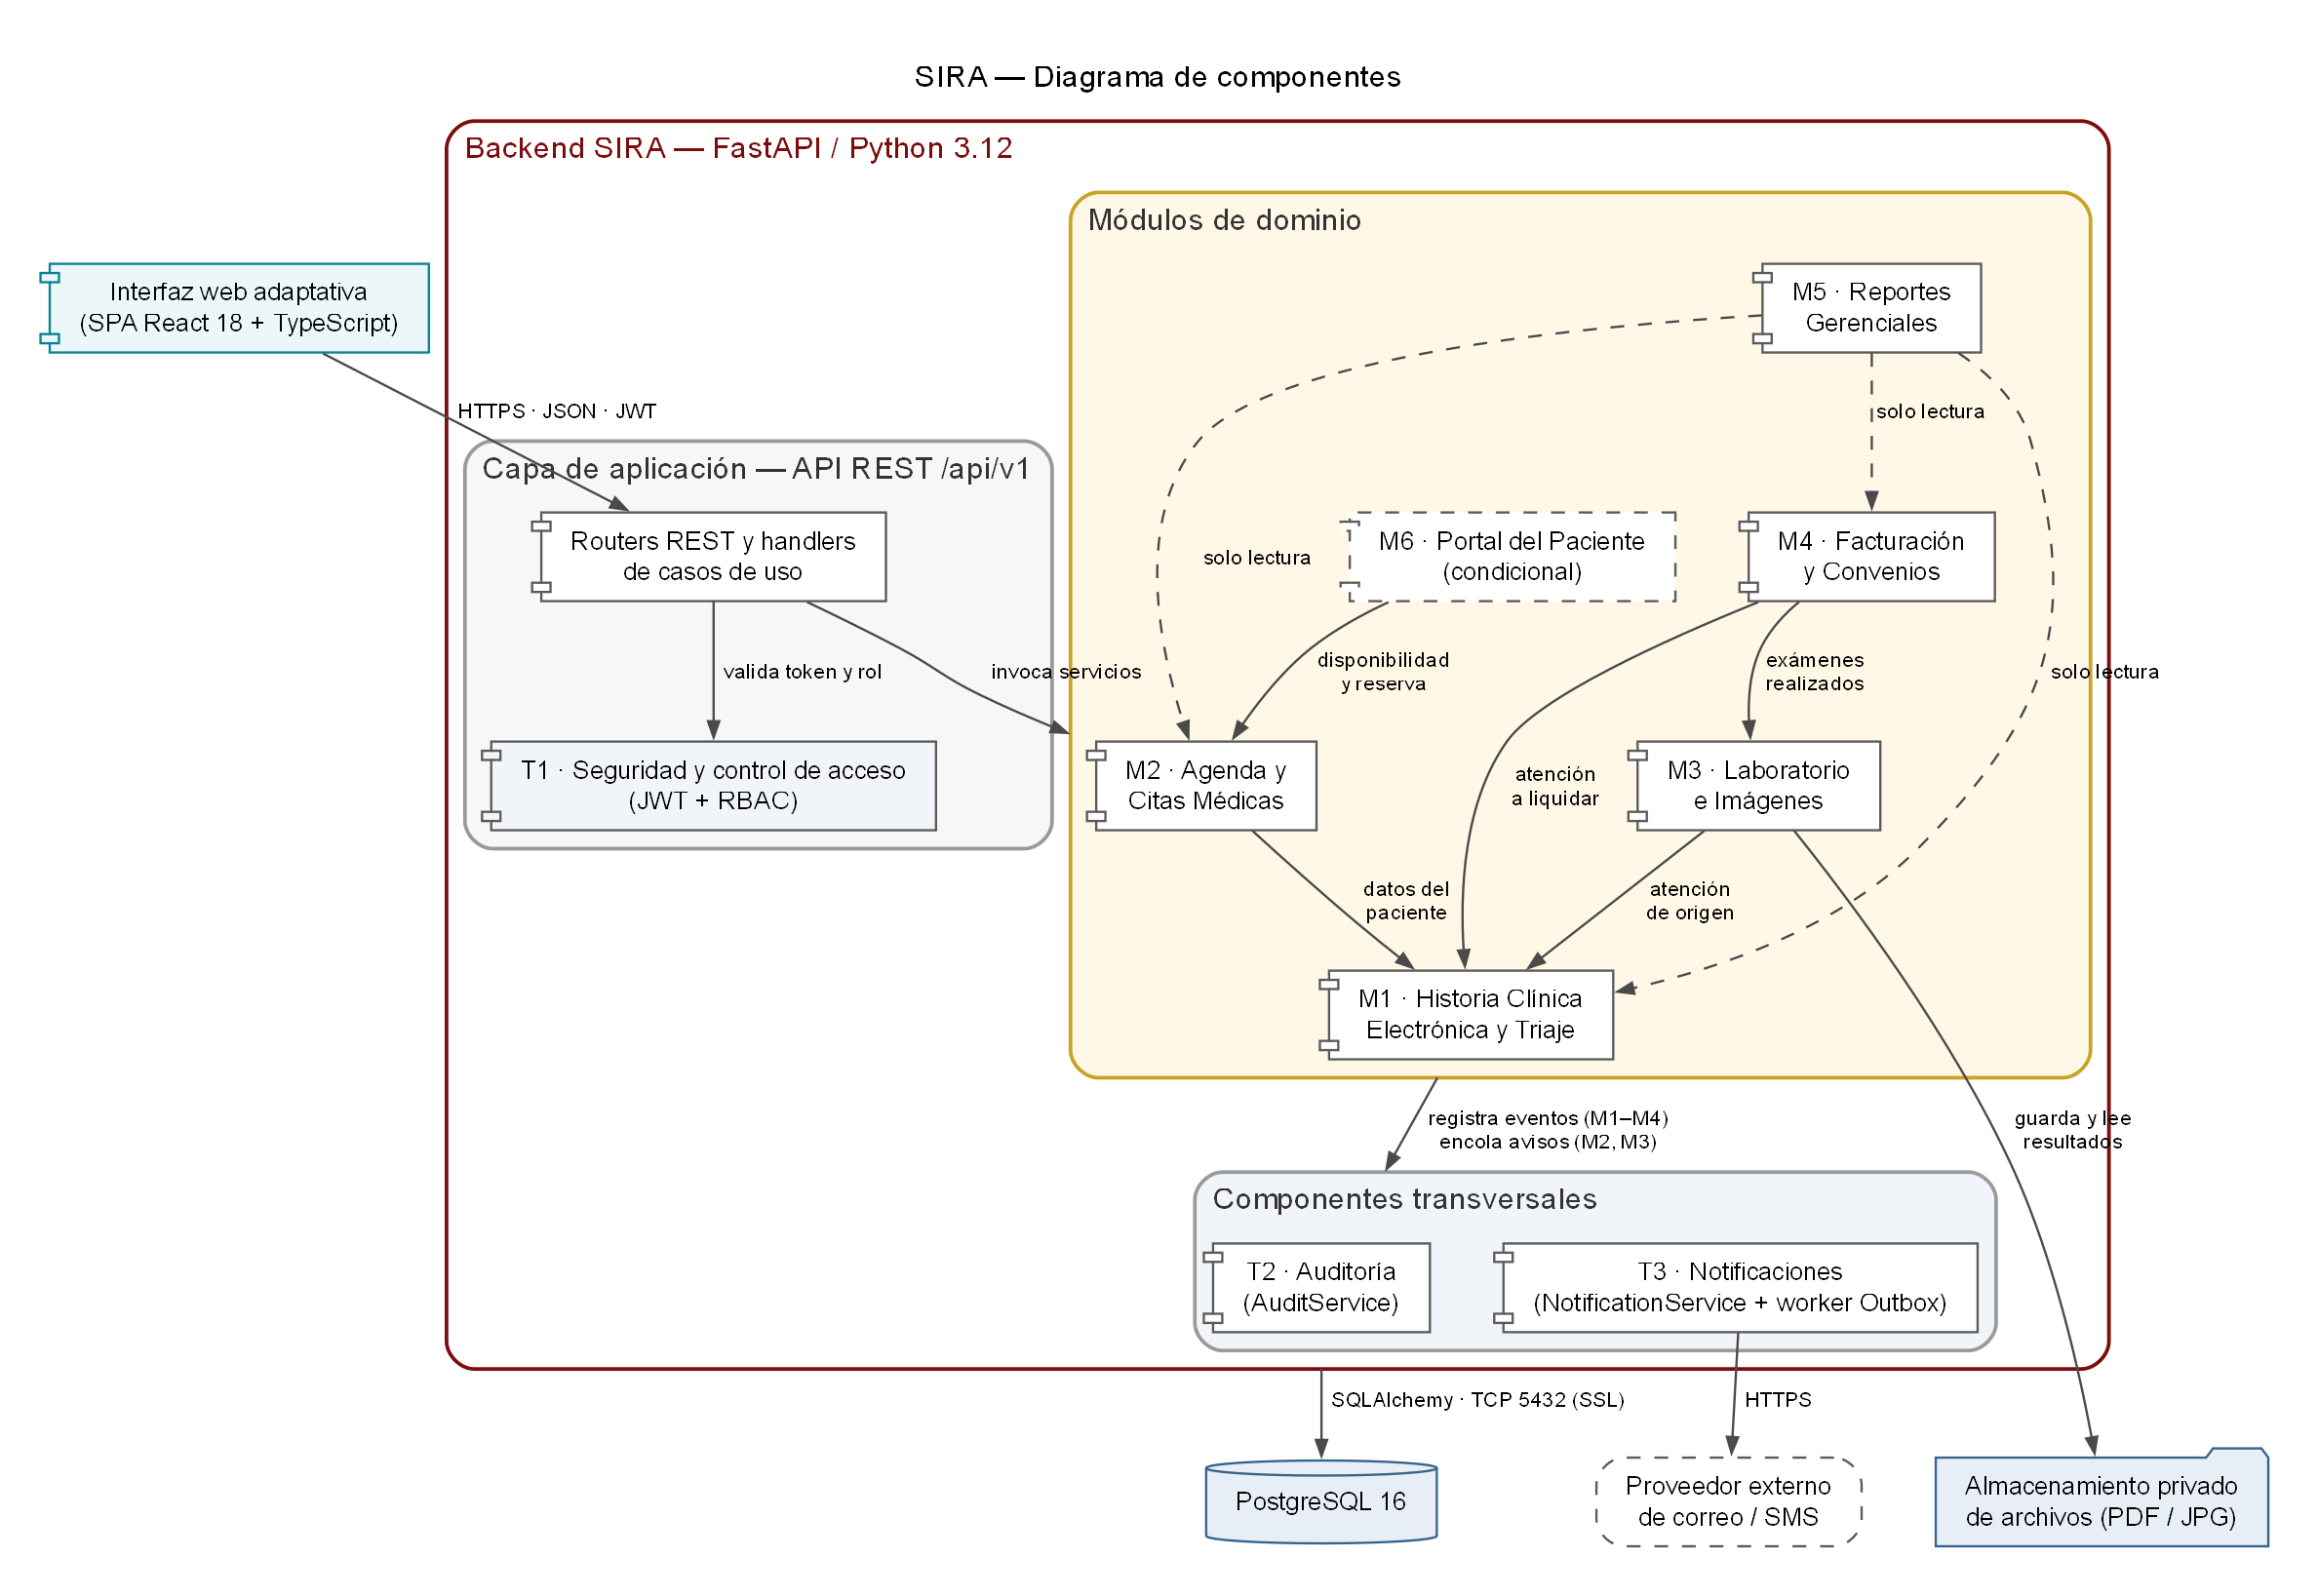
\includegraphics[width=\linewidth,height=0.75\textheight,keepaspectratio]{diagrama-componentes.png}
  \caption{Diagrama de componentes del sistema SIRA}
  \label{fig:componentes}
  {\small Versión en alta resolución en el \href{https://github.com/francito69/SW705U-grupo-A/blob/main/docs/entregable-4/diagrama-componentes.png}{repositorio de GitHub}.}
\end{figure}

\subsection{Detalle de las interfaces}

% Las rutas se derivan de las historias de usuario (ERS 3.7), los casos de uso
% (04-modelosUML.md), los prototipos (07) y la vista de desarrollo del SAD.
% El SAD solo fija literalmente POST /api/v1/citas (diagrama de secuencia S2).
\begingroup\small
\begin{xltabular}{\linewidth}{|P{5.1cm}|L|P{1.5cm}|P{2.8cm}|}
  \caption{Operaciones que expone cada componente}\label{tab:interfaces}\\
  \hline
  \rowcolor{guinda}\cab{Interfaz} & \cab{Qué hace} & \cab{HU} & \cab{Rol autorizado} \\ \hline
  \endfirsthead
  \hline
  \rowcolor{guinda}\cab{Interfaz} & \cab{Qué hace} & \cab{HU} & \cab{Rol autorizado} \\ \hline
  \endhead
  \grupo{M1 --- Historia Clínica Electrónica y Triaje}
  \ep{GET}{/pacientes} & Busca un paciente por tipo y número de documento. & HU03 & Admisión, Médico, Enfermera \\ \hline
  \ep{POST}{/pacientes} & Registra un paciente nuevo con su convenio; responde 409 si el documento ya existe. & HU03 & Admisión \\ \hline
  \ep{GET}{/pacientes/\{id\}/hce} & Devuelve el expediente cronológico (antecedentes, alergias, triajes, atenciones y resultados), paginado de 10 en 10. & HU01 & Médico; Enfermera (solo triaje y alergias) \\ \hline
  \ep{POST}{/triajes} & Registra los signos vitales de la atención del día y marca una alerta si la presión o la temperatura están fuera de rango. & HU05 & Enfermera \\ \hline
  \ep{POST}{/atenciones} & Registra la atención con diagnóstico CIE-10 obligatorio, indicaciones y receta. & HU04 & Médico \\ \hline
  \ep{GET}{/atenciones/\{id\}} & Muestra el detalle de una atención con su receta (botón ``Ver detalle'' de la HCE). & HU01, HU04 & Médico \\ \hline
  \ep{POST}{/atenciones/\{id\}/anular} & Anula la atención con un motivo de al menos 20 caracteres; el registro se conserva. & HU08 & Médico auditor, Gerencia médica \\ \hline
  \ep{GET}{/diagnosticos-cie10} & Autocompleta diagnósticos por código o descripción. & HU04 & Médico \\ \hline
  \grupo{M2 --- Agenda y Citas Médicas}
  \ep{GET}{/medicos} & Lista los médicos activos por especialidad para los filtros de la agenda. & HU02 & Admisión \\ \hline
  \ep{GET}{/citas/disponibilidad} & Lista los bloques libres por especialidad, médico y fecha. & HU02 & Admisión \\ \hline
  \ep{GET}{/citas} & Agenda del día por médico o consultorio, y lista de espera para el triaje. & HU02, HU05 & Admisión, Médico, Enfermera \\ \hline
  \ep{POST}{/citas} & Reserva la cita y encola su recordatorio en una sola transacción; responde 201, o 409 si el médico o el consultorio ya están ocupados. & HU02, HU07 & Admisión \\ \hline
  \ep{POST}{/citas/\{id\}/reprogramar} & Libera el bloque anterior y crea la nueva cita enlazada, con su recordatorio. & HU06 & Admisión \\ \hline
  \ep{POST}{/citas/\{id\}/cancelar} & Cancela la cita con motivo obligatorio y libera el bloque. & HU06 & Admisión \\ \hline
  \ep{POST}{/citas/\{id\}/check-in} & Registra la llegada del paciente y lo pasa a la lista de espera de enfermería. & HU05 & Admisión \\ \hline
  \grupo{M3 --- Laboratorio e Imágenes}
  \ep{POST}{/ordenes} & Emite una orden de examen vinculada a la atención, en estado Solicitado. & HU09 & Médico \\ \hline
  \ep{GET}{/ordenes} & Bandeja de órdenes por estado, o por paciente para mostrarlas en la HCE. & HU09 & Laboratorio, Médico \\ \hline
  \ep{PATCH}{/ordenes/\{id\}/estado} & Cambia el estado de la orden (Solicitado $\rightarrow$ En proceso). & HU10 & Laboratorio \\ \hline
  \ep{POST}{/ordenes/\{id\}/resultado} & Sube el archivo PDF/JPG con su informe, guarda su hash SHA-256 y completa la orden. & HU10 & Laboratorio \\ \hline
  \ep{GET}{/resultados/\{id\}/archivo} & Entrega el archivo mediante un enlace firmado y temporal. & HU10 & Médico \\ \hline
  \grupo{M4 --- Facturación y Convenios}
  \ep{GET}{/convenios} & Catálogo de convenios vigentes: Particular, EPS 1--5 y SOAT. & HU03, HU11 & Admisión, Caja \\ \hline
  \ep{GET}{/servicios} & Catálogo de servicios médicos y exámenes. & HU09, HU11 & Médico, Caja \\ \hline
  \ep{GET}{/tarifas/copago} & Calcula la cobertura y el copago estimados para un servicio y un convenio. & HU02, HU11 & Admisión, Caja \\ \hline
  \ep{POST}{/facturas} & Emite el comprobante interno aplicando el tarifario vigente del convenio. & HU11 & Caja \\ \hline
  \ep{POST}{/facturas/\{id\}/glosas} & Registra una glosa con su código, motivo e importe observado. & HU12 & Caja \\ \hline
  \ep{PATCH}{/glosas/\{id\}/estado} & Avanza la glosa: Registrada $\rightarrow$ Sustentada $\rightarrow$ Aceptada o Recuperada. & HU12 & Caja \\ \hline
  \grupo{M5 --- Reportes Gerenciales}
  \ep{GET}{/reportes/indicadores} & Ocupación, tiempo de espera, no-show e ingresos por rango de fechas, especialidad y convenio. & HU13 & Gerencia \\ \hline
  \ep{GET}{/reportes/ocupacion} & Ocupación de cada uno de los 12 consultorios. & HU13 & Gerencia \\ \hline
  \ep{GET}{/reportes/ingresos} & Ingresos y glosas por convenio y especialidad. & HU13 & Gerencia \\ \hline
  \grupo{M6 --- Portal del Paciente (condicional)}
  \ep{GET}{/portal/disponibilidad} & Muestra al paciente los horarios libres, usando el servicio de M2. & HU14 & Paciente \\ \hline
  \ep{POST}{/portal/citas} & Agenda la cita con las mismas validaciones de M2 y programa su recordatorio. & HU14 & Paciente \\ \hline
  \ep{GET}{/portal/mis-citas} & Lista las citas del paciente autenticado. & HU14 & Paciente \\ \hline
  \grupo{T1 --- Seguridad y control de acceso}
  \ep{POST}{/auth/login} & Valida las credenciales (contraseña con bcrypt) y entrega un token JWT con el rol. & Todas & Todos los usuarios \\ \hline
  \ep{GET}{/auth/me} & Devuelve el usuario y el rol de la sesión para armar el menú. & Todas & Usuario autenticado \\ \hline
  \grupo{T2 --- Auditoría}
  {\footnotesize\texttt{AuditService.registrar()}} & Guarda en la bitácora el usuario, la acción, la tabla, el registro, la IP, la fecha y el motivo. La invocan M1, M2, M3 y M4. & HU01, HU08 & Uso interno \\ \hline
  \grupo{T3 --- Notificaciones}
  {\footnotesize\texttt{NotificationService.encolar()}} & Guarda el mensaje en la cola Outbox dentro de la misma transacción del módulo que lo pide. & HU07, HU10 & Uso interno \\ \hline
  Proceso en segundo plano & Cada 60 s envía los mensajes pendientes por correo o SMS y registra los reintentos. & HU07 & Uso interno \\ \hline
\end{xltabular}
\endgroup

\subsection{Propiedad de datos y comunicación entre módulos}

La comunicación entre módulos sigue cuatro reglas:

\begin{enumerate}[nosep]
  \item Cada tabla tiene un único módulo dueño.
  \item Las llaves foráneas entre tablas de distintos módulos se mantienen en la base de datos para
        preservar la integridad referencial (una sola instancia de PostgreSQL, ADR-02), pero el
        código de un módulo nunca consulta ni modifica las tablas de otro: usa la operación pública
        del módulo dueño.
  \item Las dependencias van en un solo sentido, sin ciclos: M6 $\rightarrow$ M2 $\rightarrow$ M1
        $\leftarrow$ M3 $\leftarrow$ M4. M5 solo lee, y todos usan los componentes transversales.
  \item Cuando una pantalla necesita datos en sentido contrario (por ejemplo, la HCE con los
        resultados de laboratorio, o el nombre del convenio en la cabecera del paciente), los combina
        la capa de aplicación, que orquesta los servicios sin que un módulo de dominio dependa de otro.
\end{enumerate}

\begin{xltabular}{\linewidth}{|P{2.9cm}|P{4.6cm}|L|}
  \caption{Tablas que administra cada módulo y datos que consume de otros}\label{tab:propiedad}\\
  \hline
  \rowcolor{guinda}\cab{Módulo} & \cab{Tablas que administra} & \cab{Datos que consume de otros módulos (y por qué interfaz)} \\ \hline
  \endfirsthead
  \hline
  \rowcolor{guinda}\cab{Módulo} & \cab{Tablas que administra} & \cab{Datos que consume de otros módulos (y por qué interfaz)} \\ \hline
  \endhead
  M1 --- HCE y Triaje &
    \texttt{pacientes}, \texttt{atenciones}, \texttt{triajes}, \tb{diagnosticos\_cie10},
    \tb{atencion\_diagnosticos}, \texttt{prescripciones} &
    Ningún otro módulo de dominio; solo registra los accesos en T2. La vista de la HCE la arma
    la capa de aplicación con datos de M2 (médico de cada atención) y de M3 (resultados). \\ \hline
  M2 --- Agenda y Citas &
    \texttt{citas}, \texttt{medicos}, \texttt{especialidades}, \texttt{consultorios} &
    Datos del paciente (M1: \ep{GET}{/pacientes}); recordatorio de 24 h
    (T3: {\footnotesize\texttt{NotificationService.encolar()}}); registro de cambios (T2). El copago
    estimado del paso 3 de la reserva lo pide la interfaz web a M4 (\ep{GET}{/tarifas/copago}). \\ \hline
  M3 --- Laboratorio e Imágenes &
    \tb{ordenes\_examen}, \texttt{resultados} &
    Atención de origen (M1: \ep{GET}{/atenciones/\{id\}}); aviso de resultado listo (T3); registro
    de cambios (T2). La lista de exámenes que ve el médico la toma la interfaz web de M4
    (\ep{GET}{/servicios}). \\ \hline
  M4 --- Facturación y Convenios &
    \texttt{convenios}, \tb{servicios\_medicos}, \tb{tarifarios\_servicios},
    \texttt{facturas}, \tb{factura\_detalle}, \texttt{glosas} &
    Atención a liquidar (M1: \ep{GET}{/atenciones/\{id\}}); exámenes realizados
    (M3: \ep{GET}{/ordenes}); registro de glosas (T2). \\ \hline
  M5 --- Reportes Gerenciales &
    Ninguna propia (solo lectura) &
    Agregados de citas, asistencia y espera (M2); hora de inicio de la atención (M1); ingresos
    y glosas (M4). Los obtiene mediante consultas de solo lectura que publica cada módulo. \\ \hline
  M6 --- Portal del Paciente &
    Ninguna propia &
    Disponibilidad y reserva (M2: \ep{GET}{/citas/disponibilidad}, \ep{POST}{/citas});
    identidad del paciente (T1). \\ \hline
  T1 --- Seguridad y control de acceso &
    \texttt{usuarios}, \texttt{roles} &
    Ninguno: los demás módulos lo usan para validar el rol. \\ \hline
  T2 --- Auditoría &
    \tb{bitacora\_auditoria} &
    Ninguno: recibe los eventos de M1, M2, M3 y M4. \\ \hline
  T3 --- Notificaciones &
    \tb{outbox\_notificaciones} &
    Ninguno: el módulo que encola entrega el destinatario y el mensaje. El envío sale al
    proveedor externo de correo/SMS por HTTPS. \\ \hline
\end{xltabular}

% =============================================================================
\newpage
\section{Modelo de base de datos}\label{sec:modelo}

\subsection{Transformación de clases a tablas}

% Clase entre parentesis = tabla que sale de un atributo de esa clase al normalizar.
\begingroup\small
\begin{xltabular}{\linewidth}{|P{3.1cm}|P{3.2cm}|P{4cm}|L|}
  \caption{Transformación de las clases del modelo a tablas}\label{tab:clases-tablas}\\
  \hline
  \rowcolor{guinda}\cab{Clase del modelo} & \cab{Tabla} & \cab{Llave primaria / foráneas} & \cab{Restricciones} \\ \hline
  \endfirsthead
  \hline
  \rowcolor{guinda}\cab{Clase del modelo} & \cab{Tabla} & \cab{Llave primaria / foráneas} & \cab{Restricciones} \\ \hline
  \endhead
  Paciente & \texttt{pacientes} &
    PK id\_paciente \newline FK id\_convenio &
    UQ (tipo\_documento, numero\_documento); CHECK tipo\_documento y sexo \\ \hline
  Convenio & \texttt{convenios} &
    PK id\_convenio &
    UQ codigo\_convenio; CHECK tipo\_convenio: PARTICULAR, EPS, SOAT \\ \hline
  Convenio (porcentaje\_cubierto, copago\_fijo) & \tb{tarifarios\_servicios} &
    PK id\_tarifario \newline FK id\_servicio, id\_convenio &
    Cobertura de 0 a 100~\%; montos $\geq 0$; EXCLUDE: sin vigencias superpuestas para un mismo servicio y convenio \\ \hline
  OrdenExamen (nombre\_prueba, tipo\_examen) & \tb{servicios\_medicos} &
    PK id\_servicio &
    UQ codigo\_servicio; CHECK tipo\_servicio; precio $\geq 0$ \\ \hline
  Medico & \texttt{medicos} &
    PK id\_medico \newline FK id\_especialidad, id\_usuario &
    UQ cmp; UQ id\_usuario \\ \hline
  Medico (especialidad) & \texttt{especialidades} &
    PK id\_especialidad &
    UQ nombre \\ \hline
  Consultorio & \texttt{consultorios} &
    PK id\_consultorio &
    UQ numero; piso $\geq 1$ \\ \hline
  Cita & \texttt{citas} &
    PK id\_cita \newline FK id\_paciente, id\_medico, id\_consultorio, id\_cita\_origen (UQ), creado\_por &
    EXCLUDE: sin citas activas superpuestas por médico ni por consultorio; fin $>$ inicio; CHECK estado; motivo obligatorio al cancelar o reprogramar \\ \hline
  Atencion & \texttt{atenciones} &
    PK id\_atencion \newline FK id\_paciente, id\_medico, id\_cita (UQ), anulado\_por &
    Consulta externa exige cita; FINALIZADA exige motivo de consulta; anulación exige motivo ($\geq 20$ caracteres) y usuario; sin DELETE \\ \hline
  Atencion (diagnostico\_cie10) & \tb{atencion\_diagnosticos} &
    PK (id\_atencion, codigo\_cie10) \newline FK id\_atencion, codigo\_cie10 &
    CHECK tipo: PRINCIPAL, SECUNDARIO, PRESUNTIVO; un solo PRINCIPAL por atención \\ \hline
  Atencion (descripcion\_diagnostico) & \tb{diagnosticos\_cie10} &
    PK codigo &
    descripcion NOT NULL \\ \hline
  Atencion (prescripcion\_receta) & \texttt{prescripciones} &
    PK id\_prescripcion \newline FK id\_atencion &
    Medicamento, presentación, frecuencia y duración NOT NULL \\ \hline
  Triaje & \texttt{triajes} &
    PK id\_triaje \newline FK id\_atencion (UQ), id\_enfermera &
    Rangos válidos de signos vitales, peso y talla; sistólica $>$ diastólica \\ \hline
  OrdenExamen & \tb{ordenes\_examen} &
    PK id\_orden \newline FK id\_atencion, id\_servicio &
    UQ codigo\_orden; CHECK estado \\ \hline
  Resultado & \texttt{resultados} &
    PK id\_resultado \newline FK id\_orden (UQ), id\_validador &
    hash\_archivo de 64 caracteres; fecha\_resultado $\geq$ fecha\_toma\_muestra \\ \hline
  Factura & \texttt{facturas} &
    PK id\_factura \newline FK id\_atencion (UQ), id\_convenio, creado\_por &
    UQ numero\_comprobante; CHECK estado \\ \hline
  Factura (montos) & \tb{factura\_detalle} &
    PK id\_detalle \newline FK id\_factura, id\_servicio, id\_orden (UQ) &
    cantidad $> 0$; precio $\times$ cantidad = monto cubierto + copago \\ \hline
  Glosa & \texttt{glosas} &
    PK id\_glosa \newline FK id\_factura, registrado\_por &
    monto\_glosado $> 0$; CHECK estado; ACEPTADA, RECHAZADA y RECUPERADA exigen fecha\_resolucion \\ \hline
  Notificacion & \tb{outbox\_notificaciones} &
    PK id\_notificacion \newline FK id\_cita &
    CHECK tipo\_evento, canal y estado; intentos $\geq 0$ \\ \hline
  BitacoraAuditoria & \tb{bitacora\_auditoria} &
    PK id\_auditoria \newline FK id\_usuario &
    Sin UPDATE ni DELETE; ANULAR exige motivo \\ \hline
  Usuario & \texttt{usuarios} &
    PK id\_usuario \newline FK id\_rol &
    UQ username; UQ email \\ \hline
  Rol & \texttt{roles} &
    PK id\_rol &
    UQ nombre; CHECK nombre \\ \hline
\end{xltabular}
\endgroup

\subsection{Diagrama entidad-relación}

% Fuente editable: figuras/script-img-entidas-relacion.mmd (Mermaid)
\begin{figure}[p]
  \centering
  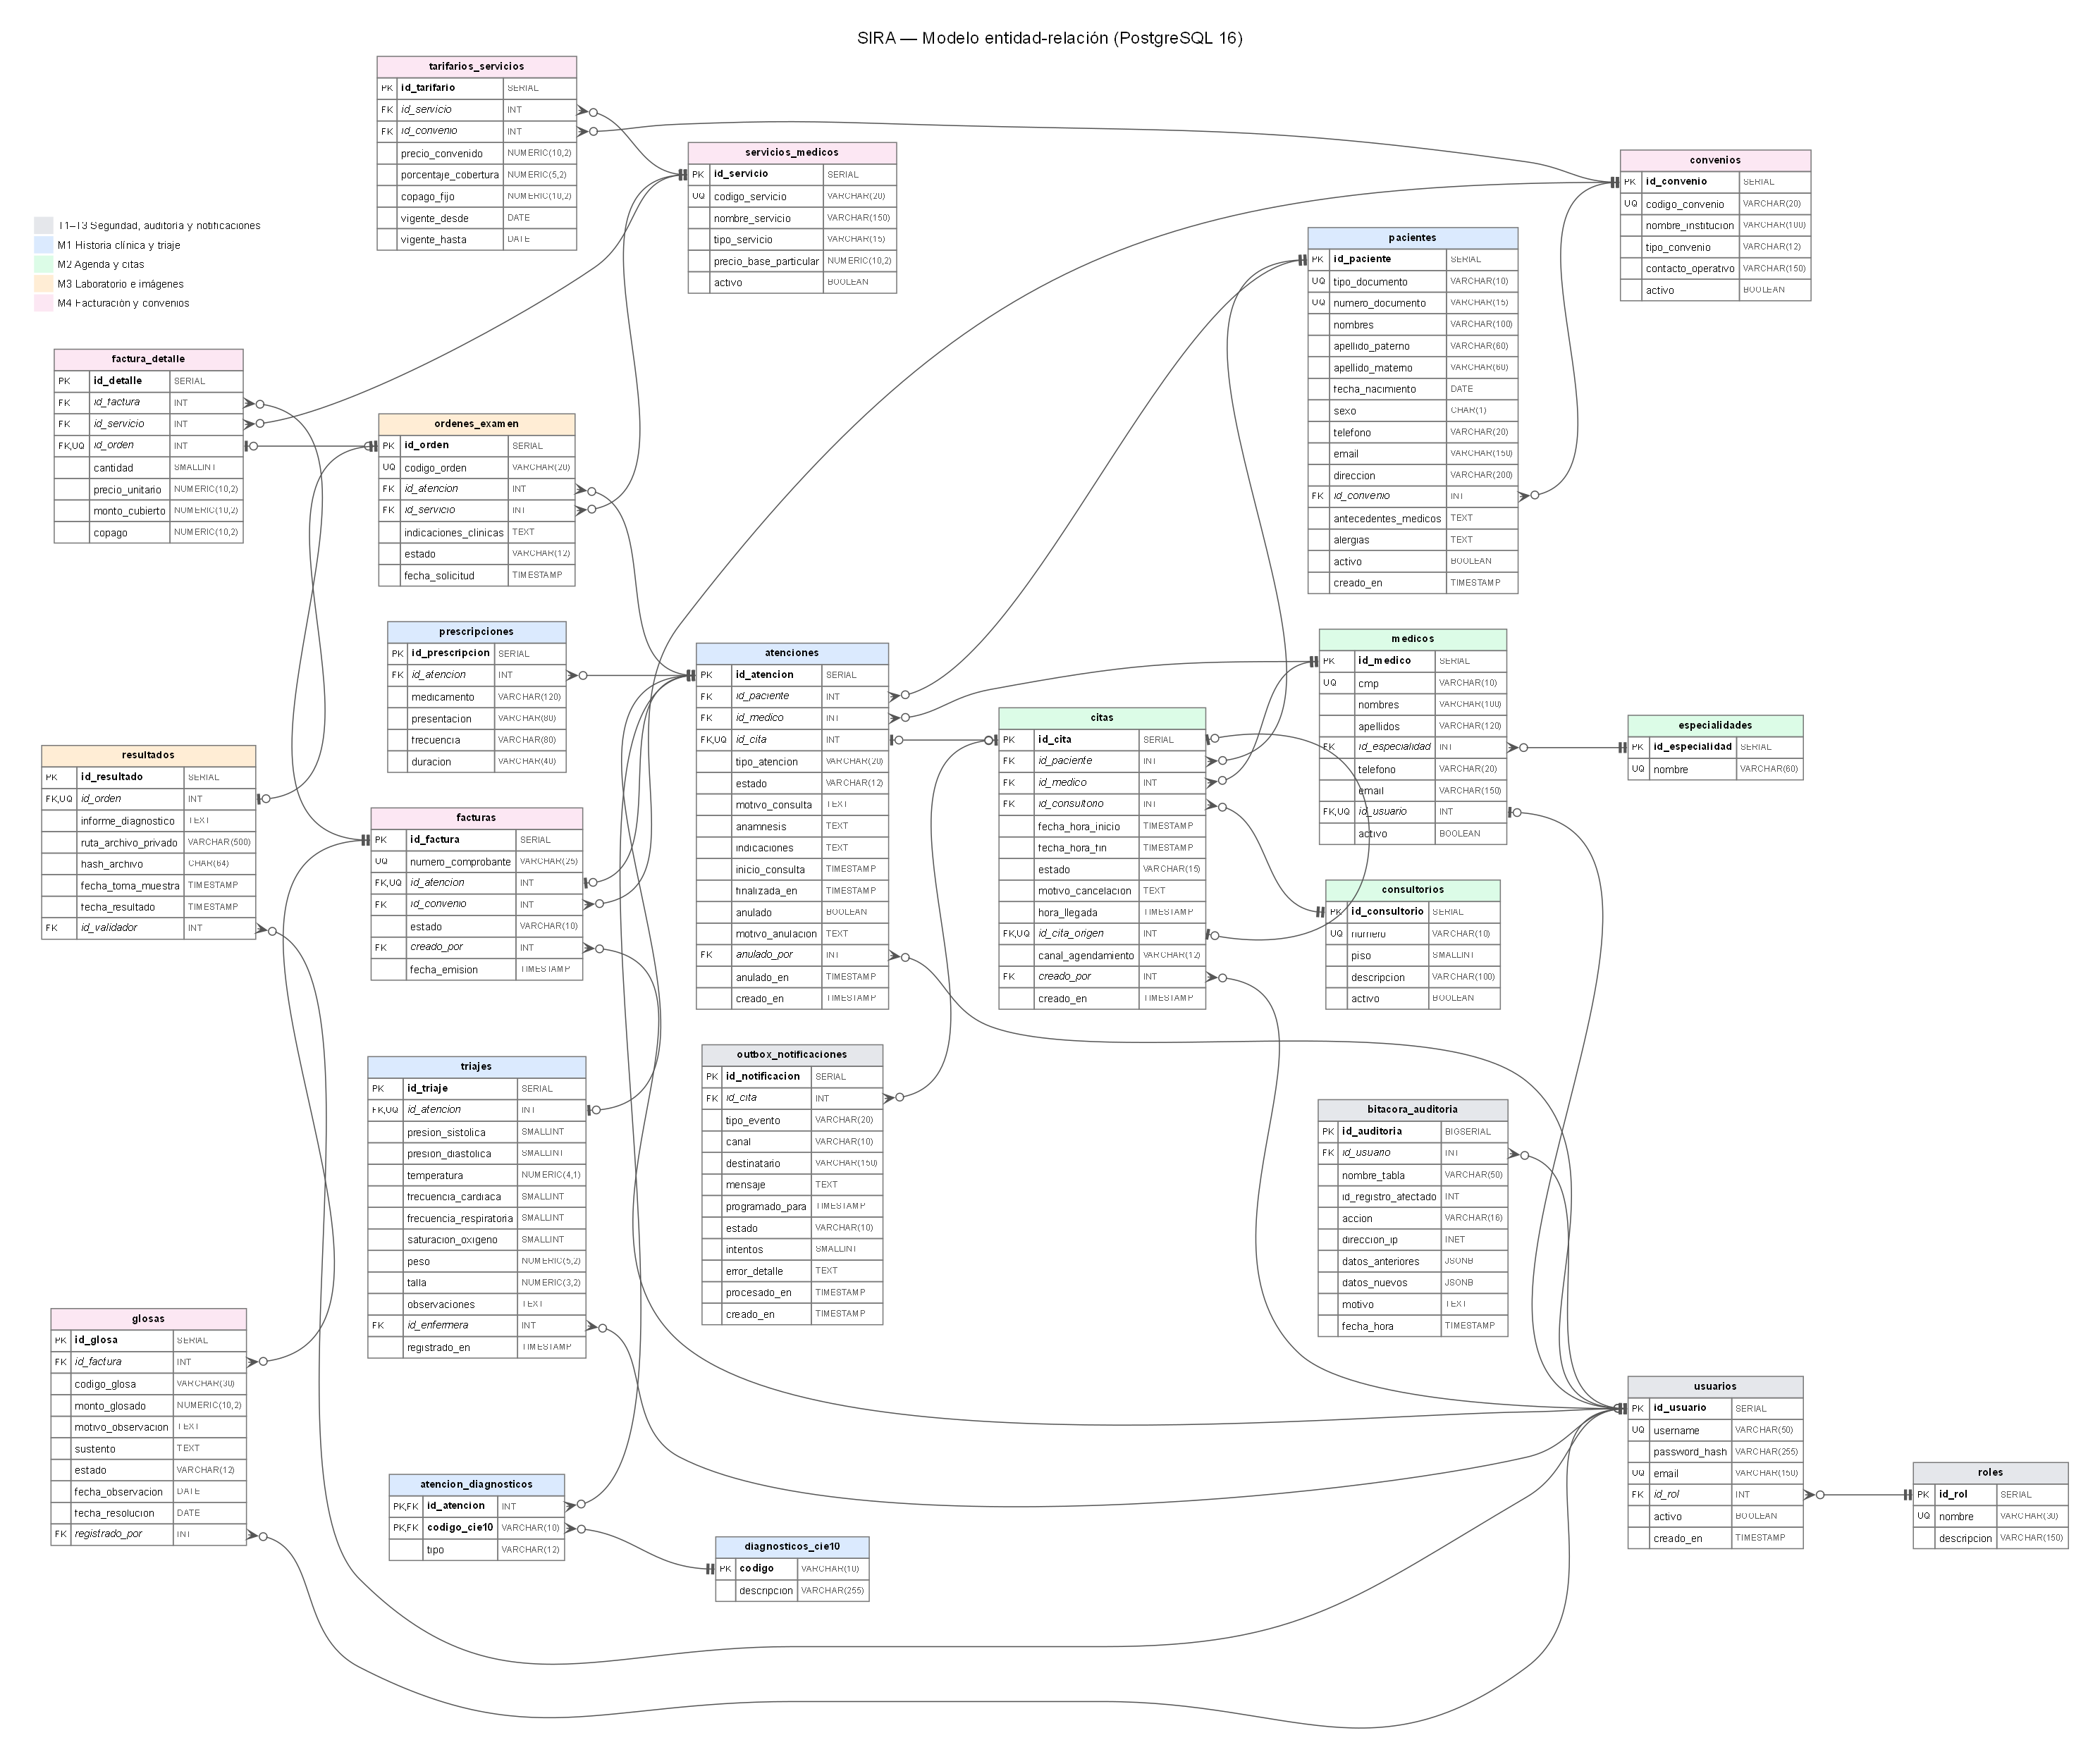
\includegraphics[width=\linewidth,height=0.85\textheight,keepaspectratio]{modelo-entidad-relacion.png}
  \caption{Modelo entidad-relación del sistema SIRA (notación pata de gallo)}
  \label{fig:mer}
  {\small Versión en alta resolución en el \href{https://github.com/francito69/SW705U-grupo-A/blob/main/docs/entregable-4/modelo-entidad-relacion.png}{repositorio de GitHub}.}
\end{figure}

\subsection{Verificación de las formas normales}

\begin{xltabular}{\linewidth}{|P{1.6cm}|P{4.6cm}|L|}
  \caption{Verificación de 1FN, 2FN y 3FN}\label{tab:formas-normales}\\
  \hline
  \rowcolor{guinda}\cab{Forma normal} & \cab{Criterio} & \cab{Cómo lo cumple el modelo} \\ \hline
  \endfirsthead
  \hline
  \rowcolor{guinda}\cab{Forma normal} & \cab{Criterio} & \cab{Cómo lo cumple el modelo} \\ \hline
  \endhead
  1FN & Valores atómicos, sin grupos repetitivos en una misma columna. &
    Una fila por medicamento (\texttt{prescripciones}) y por diagnóstico
    (\tb{atencion\_diagnosticos}); presión sistólica y diastólica en columnas separadas;
    apellido paterno y materno separados. \\ \hline
  2FN & Cumple 1FN y ningún atributo depende solo de una parte de una llave compuesta. &
    En \tb{atencion\_diagnosticos}, \texttt{tipo} depende de la llave completa. Precio,
    cobertura y copago dependen del servicio y del convenio (\tb{tarifarios\_servicios});
    \tb{precio\_base\_particular} depende solo del servicio (\tb{servicios\_medicos}). \\ \hline
  3FN & Cumple 2FN y ningún atributo no clave depende de otro atributo no clave. &
    Especialidad y descripción del diagnóstico en catálogos propios; el IMC no se almacena;
    los montos del comprobante se registran por línea en \tb{factura\_detalle}. \\ \hline
\end{xltabular}

\subsection{Decisiones de normalización justificadas}

\begin{xltabular}{\linewidth}{|P{0.7cm}|P{3.6cm}|P{1.8cm}|L|}
  \caption{Decisiones de normalización}\label{tab:decisiones}\\
  \hline
  \rowcolor{guinda}\cab{N.°} & \cab{Decisión} & \cab{Forma normal} & \cab{Justificación} \\ \hline
  \endfirsthead
  \hline
  \rowcolor{guinda}\cab{N.°} & \cab{Decisión} & \cab{Forma normal} & \cab{Justificación} \\ \hline
  \endhead
  1 & Tabla \texttt{prescripciones} & 1FN &
    \tb{prescripcion\_receta} guardaba varios medicamentos en un solo texto. \\ \hline
  2 & Tabla \tb{tarifarios\_servicios} con vigencia & 2FN &
    Cobertura y copago dependen del par servicio--convenio, no solo del convenio. \\ \hline
  3 & Catálogos \texttt{especialidades} y \tb{diagnosticos\_cie10} & 3FN &
    El nombre de la especialidad se repetía en cada médico, y la descripción del diagnóstico
    depende del código CIE-10, no de la atención. \\ \hline
  4 & IMC sin columna & 3FN &
    Depende de peso y talla; se calcula al consultar. \\ \hline
  5 & Anulación lógica & Negocio (RNF-004) &
    Las tablas clínicas no admiten DELETE; \texttt{atenciones} registra anulación, motivo,
    usuario y fecha. \\ \hline
\end{xltabular}

% =============================================================================
\newpage
\section{Script SQL y datos de prueba}\label{sec:script}

\subsection{Motor y archivos del script}

\begin{xltabular}{\linewidth}{|P{4.5cm}|L|}
  \caption{Motor de base de datos y ubicación de los scripts}\label{tab:archivos-sql}\\
  \hline
  \rowcolor{guinda}\cab{Elemento} & \cab{Detalle} \\ \hline
  \endfirsthead
  \hline
  \rowcolor{guinda}\cab{Elemento} & \cab{Detalle} \\ \hline
  \endhead
  Motor de base de datos     & PostgreSQL 16 (decisión ADR-02 del SAD), extensión \tb{btree\_gist}; pruebas ejecutadas en PostgreSQL 18 con pgAdmin~4 \\ \hline
  Script de creación         & \nolinkurl{database/01-esquema.sql}: 22 tablas, restricciones, índices, triggers y una vista \\ \hline
  Script de datos de prueba  & \nolinkurl{database/02-datos-prueba.sql} \\ \hline
  Script de verificación     & \nolinkurl{database/03-verificacion.sql}: conteo de registros y 10 pruebas de restricciones \\ \hline
  Enlace al repositorio      & \url{https://github.com/francito69/SW705U-grupo-A} \\ \hline
\end{xltabular}

\subsection{Script de creación (extracto)}

\begin{lstlisting}[style=sql, caption={Tabla \texttt{citas} y trigger contra el borrado físico (extracto de \texttt{01-esquema.sql})}, label={lst:ddl}]
CREATE EXTENSION IF NOT EXISTS btree_gist;

CREATE TABLE citas (
    id_cita            SERIAL      PRIMARY KEY,
    id_paciente        INT         NOT NULL REFERENCES pacientes (id_paciente),
    id_medico          INT         NOT NULL REFERENCES medicos (id_medico),
    id_consultorio     INT         NOT NULL REFERENCES consultorios (id_consultorio),
    fecha_hora_inicio  TIMESTAMP   NOT NULL,
    fecha_hora_fin     TIMESTAMP   NOT NULL,
    estado             VARCHAR(15) NOT NULL DEFAULT 'CONFIRMADA'
                       CHECK (estado IN ('CONFIRMADA', 'EN_ESPERA', 'ATENDIDA',
                                         'CANCELADA', 'REPROGRAMADA', 'NO_ASISTIO')),
    motivo_cancelacion TEXT,
    hora_llegada       TIMESTAMP,
    id_cita_origen     INT         UNIQUE REFERENCES citas (id_cita),
    canal_agendamiento VARCHAR(12) NOT NULL DEFAULT 'ADMISION'
                       CHECK (canal_agendamiento IN ('ADMISION', 'PORTAL_WEB', 'TELEFONICO')),
    creado_por         INT         NOT NULL REFERENCES usuarios (id_usuario),
    creado_en          TIMESTAMP   NOT NULL DEFAULT CURRENT_TIMESTAMP,
    CONSTRAINT chk_cita_rango CHECK (fecha_hora_fin > fecha_hora_inicio),
    CONSTRAINT chk_cita_motivo CHECK (
        estado NOT IN ('CANCELADA', 'REPROGRAMADA') OR motivo_cancelacion IS NOT NULL),
    CONSTRAINT chk_cita_llegada CHECK (
        estado NOT IN ('EN_ESPERA', 'ATENDIDA') OR hora_llegada IS NOT NULL),
    CONSTRAINT no_solapamiento_medico EXCLUDE USING gist (
        id_medico WITH =,
        tsrange(fecha_hora_inicio, fecha_hora_fin) WITH &&
    ) WHERE (estado IN ('CONFIRMADA', 'EN_ESPERA')),
    CONSTRAINT no_solapamiento_consultorio EXCLUDE USING gist (
        id_consultorio WITH =,
        tsrange(fecha_hora_inicio, fecha_hora_fin) WITH &&
    ) WHERE (estado IN ('CONFIRMADA', 'EN_ESPERA'))
);

CREATE FUNCTION impedir_borrado() RETURNS trigger AS $$
BEGIN
    RAISE EXCEPTION 'No se permite eliminar registros de %: use la anulación lógica (RNF-004)',
        TG_TABLE_NAME
        USING ERRCODE = 'restrict_violation';
END;
$$ LANGUAGE plpgsql;

CREATE TRIGGER trg_atenciones_sin_borrado BEFORE DELETE ON atenciones
    FOR EACH ROW EXECUTE FUNCTION impedir_borrado();
\end{lstlisting}

\subsection{Script de datos de prueba (extracto)}

\begin{lstlisting}[style=sql, caption={Médicos y detalle de comprobantes (extracto de \texttt{02-datos-prueba.sql})}, label={lst:inserts}]
INSERT INTO medicos (cmp, nombres, apellidos, id_especialidad, telefono, email, id_usuario) VALUES
    ('39412', 'Jorge',    'Valdivia Ríos',  2, '987600001', 'jvaldivia@sanrafael.test', 3),
    ('48921', 'Carlos',   'Mendoza Salas',  3, '987600002', 'cmendoza@sanrafael.test',  4),
    ('31877', 'Alberto',  'Ramos Peña',     1, '987600003', 'aramos@sanrafael.test',    5),
    ('52310', 'Patricia', 'Soto Lazo',      6, '987600004', 'psoto@sanrafael.test',     6),
    ('44108', 'Mónica',   'Morales Vidal',  4, '987600005', 'mmorales@sanrafael.test',  7),
    ('50733', 'Luis',     'Torres Campos',  5, '987600006', 'ltorres@sanrafael.test',   8);

INSERT INTO factura_detalle (id_factura, id_servicio, id_orden, cantidad, precio_unitario, monto_cubierto, copago) VALUES
    (1, 1, NULL, 1,  80.00,  48.00, 32.00),
    (2, 1, NULL, 1,  80.00,  48.75, 31.25),
    (2, 3, 5,    1,  35.00,  26.25,  8.75),
    (3, 2, NULL, 1, 140.00,  96.00, 44.00),
    (3, 8, 3,    1, 120.00,  96.00, 24.00),
    (4, 9, NULL, 1, 100.00, 100.00,  0.00),
    (4, 7, 4,    1,  90.00,  90.00,  0.00),
    (5, 2, NULL, 1, 140.00,  97.75, 42.25),
    (5, 5, 1,    1,  60.00,  51.00,  9.00),
    (5, 4, 2,    1,  15.00,  12.75,  2.25);
\end{lstlisting}

\subsection{Resumen de los datos de prueba}

Todos los registros son ficticios y fueron creados para este proyecto; no corresponden a
pacientes, médicos ni personal reales.

\begingroup\small
\begin{xltabular}{\linewidth}{|P{4.4cm}|P{1.7cm}|L|}
  \caption{Registros de prueba por tabla}\label{tab:datos-prueba}\\
  \hline
  \rowcolor{guinda}\cab{Tabla} & \cab{Registros} & \cab{Datos ficticios} \\ \hline
  \endfirsthead
  \hline
  \rowcolor{guinda}\cab{Tabla} & \cab{Registros} & \cab{Datos ficticios} \\ \hline
  \endhead
  \texttt{pacientes}             & 10 & DNI y CE, con convenio particular, EPS y SOAT; alergias y antecedentes \\ \hline
  \texttt{medicos}               &  6 & Seis especialidades, cada uno con su usuario \\ \hline
  \texttt{citas}                 & 11 & Todos los estados: confirmada, en espera, atendida, cancelada, reprogramada y no asistió \\ \hline
  \texttt{atenciones}            &  7 & Consulta externa y tópico de urgencias; una en curso y una anulada con motivo \\ \hline
  \texttt{triajes}               &  6 & Signos vitales; uno con presión elevada \\ \hline
  \tb{atencion\_diagnosticos} & 8 & Diagnósticos principal, secundario y presuntivo \\ \hline
  \texttt{prescripciones}        &  7 & Medicamento, presentación, frecuencia y duración \\ \hline
  \tb{ordenes\_examen}       &  7 & Laboratorio e imágenes en estados solicitado, en proceso y completado \\ \hline
  \texttt{resultados}            &  5 & Informe, ruta privada, hash SHA-256 y entrega en menos de 4 horas \\ \hline
  \tb{tarifarios\_servicios} & 14 & Particular, tres EPS y SOAT; una tarifa histórica con vigencia cerrada \\ \hline
  \texttt{facturas}              &  5 & Emitidas, pagadas y observadas \\ \hline
  \tb{factura\_detalle}      & 10 & Consultas, exámenes y tópico; monto cubierto + copago = precio \\ \hline
  \texttt{glosas}                &  5 & Los cinco estados: registrada, sustentada, aceptada, rechazada y recuperada \\ \hline
  \tb{outbox\_notificaciones} & 7 & Recordatorios, confirmación y aviso de resultado; pendientes, enviados y uno fallido \\ \hline
  \tb{bitacora\_auditoria}   &  6 & Consulta, registro, actualización, anulación y acceso denegado \\ \hline
  \texttt{usuarios}              & 16 & Usuarios de prueba para los siete roles del sistema \\ \hline
  Catálogos                      & 54 & \texttt{roles} (7), \texttt{convenios} (7), \texttt{especialidades} (8),
                                       \texttt{consultorios} (12), \tb{diagnosticos\_cie10} (11),
                                       \tb{servicios\_medicos} (9) \\ \hline
\end{xltabular}
\endgroup

\subsection{Pruebas de las restricciones}

\begingroup\small
\begin{xltabular}{\linewidth}{|P{0.7cm}|L|P{4.6cm}|P{2.2cm}|}
  \caption{Operaciones inválidas ejecutadas en \texttt{03-verificacion.sql}}\label{tab:pruebas-sql}\\
  \hline
  \rowcolor{guinda}\cab{N.°} & \cab{Operación intentada} & \cab{Restricción que la impide} & \cab{Resultado} \\ \hline
  \endfirsthead
  \hline
  \rowcolor{guinda}\cab{N.°} & \cab{Operación intentada} & \cab{Restricción que la impide} & \cab{Resultado} \\ \hline
  \endhead
  1  & Cita del mismo médico en un horario ya ocupado (RF-002) & \tb{no\_solapamiento\_medico} & Rechazada \\ \hline
  2  & Cita en un consultorio ya ocupado (RF-002) & \tb{no\_solapamiento\_consultorio} & Rechazada \\ \hline
  3  & \texttt{DELETE} de una atención (RNF-004) & Trigger \tb{impedir\_borrado} & Rechazada \\ \hline
  4  & Anulación con un motivo de 5 caracteres (HU08) & \tb{chk\_atencion\_anulacion} & Rechazada \\ \hline
  5  & \texttt{UPDATE} sobre la bitácora (RNF-002) & Trigger \tb{impedir\_cambios\_bitacora} & Rechazada \\ \hline
  6  & Paciente con un DNI ya registrado (HU03) & \tb{uq\_paciente\_documento} & Rechazada \\ \hline
  7  & Segundo diagnóstico principal en una atención (HU04) & \tb{uq\_diagnostico\_principal} & Rechazada \\ \hline
  8  & Línea de comprobante con montos que no cuadran (RF-006) & \tb{chk\_detalle\_montos} & Rechazada \\ \hline
  9  & Dos tarifas vigentes a la vez para el mismo servicio y convenio (RF-006) & \tb{no\_solapamiento\_tarifario} & Rechazada \\ \hline
  10 & Triaje con presión sistólica menor que la diastólica (HU05) & \tb{chk\_triaje\_presion} & Rechazada \\ \hline
\end{xltabular}
\endgroup

\subsection{Evidencia de ejecución}

\begin{figure}[!htbp]
  \centering
  \includegraphics[width=\linewidth]{evidencia-sql-registros.png}
  \caption{Registros por tabla después de ejecutar \texttt{01-esquema.sql} y \texttt{02-datos-prueba.sql}}
  \label{fig:evidencia-registros}
\end{figure}

\begin{figure}[!htbp]
  \centering
  \includegraphics[width=\linewidth]{evidencia-sql-pruebas.png}
  \caption{Resultado de las pruebas de \texttt{03-verificacion.sql} en pgAdmin~4}
  \label{fig:evidencia-pruebas}
\end{figure}

% =============================================================================
\newpage
\section{Prototipo UX/UI}\label{sec:prototipo}

El prototipo cubre las pantallas de los módulos del Sprint~1 (M1 y M2) y el tablero gerencial
(M5), con la especificación de \nolinkurl{docs/entregable-1/07-prototipo-ux-ui/}.

\subsection{Pantallas del prototipo}

Tarea principal: \textbf{agendar una cita} (P2), con la meta de la HU02 y el RNF-005: 3 pasos y
menos de 3 minutos.

\begin{xltabular}{\linewidth}{|P{4cm}|L|L|}
  \caption{Pantallas del prototipo}\label{tab:pantallas}\\
  \hline
  \rowcolor{guinda}\cab{Pantalla} & \cab{Historia de usuario que atiende} & \cab{Tarea principal y tiempo medido} \\ \hline
  \endfirsthead
  \hline
  \rowcolor{guinda}\cab{Pantalla} & \cab{Historia de usuario que atiende} & \cab{Tarea principal y tiempo medido} \\ \hline
  \endhead
  \textbf{P1.} Registro de atención y HCE unificada \newline (Médico --- M1) &
    HU01 (consulta de la HCE), HU04 (diagnóstico CIE-10 y receta), HU08 (anulación con motivo);
    da acceso a HU09 (emitir orden) y HU10 (ver informe PDF) &
    Registrar la atención de un paciente con triaje hecho: diagnóstico CIE-10, receta y firma.
    Meta: expediente visible en $\leq 2$~s (RNF-001). \\ \hline
  \textbf{P2.} Agendamiento de citas en 3 pasos \newline (Admisión --- M2) &
    HU02 (agendar sin solapamientos), HU03 (buscar o registrar al paciente en el paso 1),
    HU07 (recordatorio de 24~h); la misma matriz sirve para reprogramar (HU06) &
    \textbf{Tarea principal:} reservar una cita para un paciente registrado. Meta: 3 pasos y
    $\leq 3$~min (HU02, RNF-005). Tiempo medido: tabla~\ref{tab:tiempo}. \\ \hline
  \textbf{P3.} Registro de triaje y signos vitales \newline (Enfermería --- M1) &
    HU05 (signos vitales con alerta fuera de rango) &
    Registrar los signos vitales de un paciente de la lista de espera y enviarlo al consultorio.
    Meta: $< 2$~min. Tiempo medido: tabla~\ref{tab:tiempo}. \\ \hline
  \textbf{P4.} Tablero gerencial de indicadores \newline (Gerencia --- M5) &
    HU13 (ocupación, espera, no-show e ingresos); estado de las glosas de la HU12 &
    Filtrar un mes y leer la ocupación de los 12 consultorios. Meta: tablero dibujado en
    $\leq 3$~s (HU13). \\ \hline
\end{xltabular}

\subsection{Wireframes de baja fidelidad}

Wireframes en escala de grises de P2, P1 y P3 (figuras \ref{fig:wf-agenda}, \ref{fig:wf-hce} y
\ref{fig:wf-triaje}). P4 pasó directamente a alta fidelidad porque solo presenta información.

\begin{figure}[!htbp]
  \centering
  \includegraphics[width=0.95\linewidth]{wireframe-agenda.png}
  \caption{Wireframe de baja fidelidad --- P2. Agendamiento de citas en 3 pasos}
  \label{fig:wf-agenda}
\end{figure}

\begin{figure}[!htbp]
  \centering
  \includegraphics[width=0.95\linewidth]{wireframe-hce.png}
  \caption{Wireframe de baja fidelidad --- P1. Registro de atención y HCE unificada}
  \label{fig:wf-hce}
\end{figure}

\begin{figure}[!htbp]
  \centering
  \includegraphics[width=0.95\linewidth]{wireframe-triaje.png}
  \caption{Wireframe de baja fidelidad --- P3. Registro de triaje y signos vitales}
  \label{fig:wf-triaje}
\end{figure}

\clearpage
\subsection{Prototipo navegable}

\begin{xltabular}{\linewidth}{|P{4.5cm}|L|}
  \caption{Datos del prototipo navegable}\label{tab:prototipo}\\
  \hline
  \rowcolor{guinda}\cab{Elemento} & \cab{Detalle} \\ \hline
  \endfirsthead
  \hline
  \rowcolor{guinda}\cab{Elemento} & \cab{Detalle} \\ \hline
  \endhead
  Herramienta utilizada & Google Stitch para las pantallas de alta fidelidad y Figma Make para el
    prototipo navegable con su modo de medición del tiempo \\ \hline
  Enlace navegable      & \url{https://zaffre-ajar-01499329.figma.site} \\ \hline
  Pantallas incluidas   & P1 a P4 (tabla~\ref{tab:pantallas}) \\ \hline
\end{xltabular}

% Sistema de diseño tomado de docs/entregable-1/07-prototipo-ux-ui/07-prototipos-ux-ui.md
\begin{xltabular}{\linewidth}{|P{3.6cm}|P{3.8cm}|L|}
  \caption{Sistema de diseño de las pantallas de alta fidelidad}\label{tab:diseno}\\
  \hline
  \rowcolor{guinda}\cab{Elemento} & \cab{Valor} & \cab{Uso} \\ \hline
  \endfirsthead
  \hline
  \rowcolor{guinda}\cab{Elemento} & \cab{Valor} & \cab{Uso} \\ \hline
  \endhead
  Azul clínico      & \muestra{0A4D68}\,\muestra{088395} \texttt{\#0A4D68}, \texttt{\#088395} &
    Barra de navegación, botones principales y títulos \\ \hline
  Cian de acento    & \muestra{05BFDB}\,\muestra{EBF7F9} \texttt{\#05BFDB}, \texttt{\#EBF7F9} &
    Selección, estados activos y consultorios disponibles \\ \hline
  Rojo de alerta    & \muestra{DC2626}\,\muestra{FEE2E2} \texttt{\#DC2626}, \texttt{\#FEE2E2} &
    Solo alergias, contraindicaciones y cancelaciones críticas \\ \hline
  Ámbar preventivo  & \muestra{F59E0B}\,\muestra{FEF3C7} \texttt{\#F59E0B}, \texttt{\#FEF3C7} &
    Pendientes, glosas observadas y citas por confirmar \\ \hline
  Verde de éxito    & \muestra{10B981}\,\muestra{D1FAE5} \texttt{\#10B981}, \texttt{\#D1FAE5} &
    Citas confirmadas, resultados completados y copagos pagados \\ \hline
  Grises y superficies & \texttt{\#F8FAFC}, \texttt{\#FFFFFF}, \texttt{\#64748B}, \texttt{\#1E293B} &
    Fondo, tarjetas, texto secundario y texto principal \\ \hline
  Tipografía        & Inter / Roboto, de 12 a 24~px &
    Lectura en monitores de consultorio y de recepción \\ \hline
\end{xltabular}

\begin{xltabular}{\linewidth}{|P{0.8cm}|P{3.2cm}|L|P{3.2cm}|}
  \caption{Flujo de navegación entre las pantallas del prototipo}\label{tab:flujo}\\
  \hline
  \rowcolor{guinda}\cab{N.°} & \cab{Pantalla de origen} & \cab{Acción del usuario} & \cab{Pantalla de destino} \\ \hline
  \endfirsthead
  \hline
  \rowcolor{guinda}\cab{N.°} & \cab{Pantalla de origen} & \cab{Acción del usuario} & \cab{Pantalla de destino} \\ \hline
  \endhead
  1 & Inicio de sesión & El usuario ingresa sus credenciales; el sistema muestra solo el menú de su rol. & Inicio según el rol \\ \hline
  2 & P2, paso 1 & Admisión busca al paciente por DNI y lo selecciona, o lo registra si no existe. & P2, paso 2 \\ \hline
  3 & P2, paso 2 & Elige especialidad, médico y un bloque libre de la matriz. & P2, paso 3 \\ \hline
  4 & P2, paso 3 & Revisa el copago, deja activo el recordatorio y pulsa ``Confirmar cita y emitir ticket''. & Ticket de la cita \\ \hline
  5 & P3 & El día de la cita, la enfermera elige el ticket en espera, registra los signos vitales y pulsa ``Guardar triaje''. & Lista de espera del médico \\ \hline
  6 & P1 & El médico abre al paciente desde su agenda, revisa alergias y triaje, registra diagnóstico y receta, y pulsa ``Firmar y finalizar''. & Agenda del médico \\ \hline
  7 & Inicio (Gerencia) & La gerencia abre el tablero y filtra por mes, especialidad o convenio. & P4 \\ \hline
\end{xltabular}

\begin{figure}[!htbp]
  \centering
  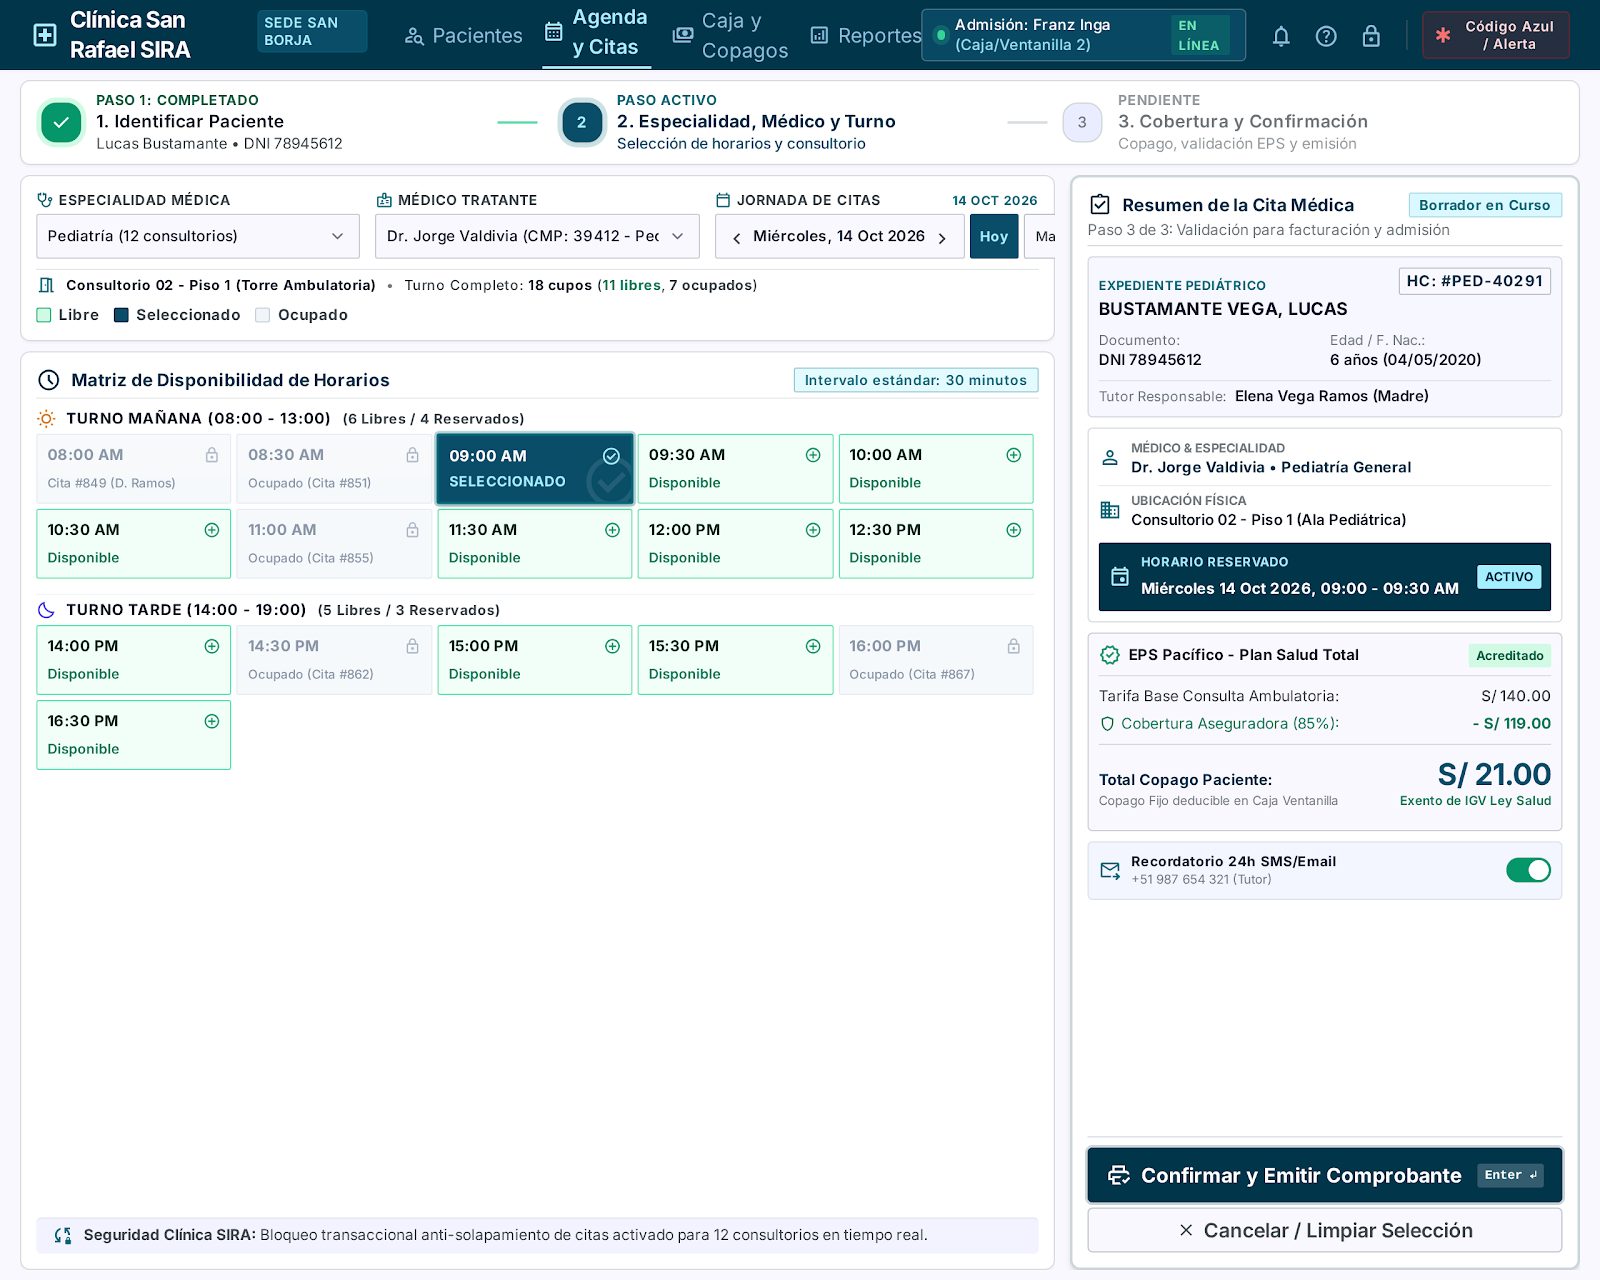
\includegraphics[width=0.95\linewidth]{AgendamientoCitasMedicas.png}
  \caption{Prototipo --- P2. Agendamiento de citas, paso 2 activo con el resumen del paso 3}
  \label{fig:proto-agenda}
\end{figure}

\begin{figure}[!htbp]
  \centering
  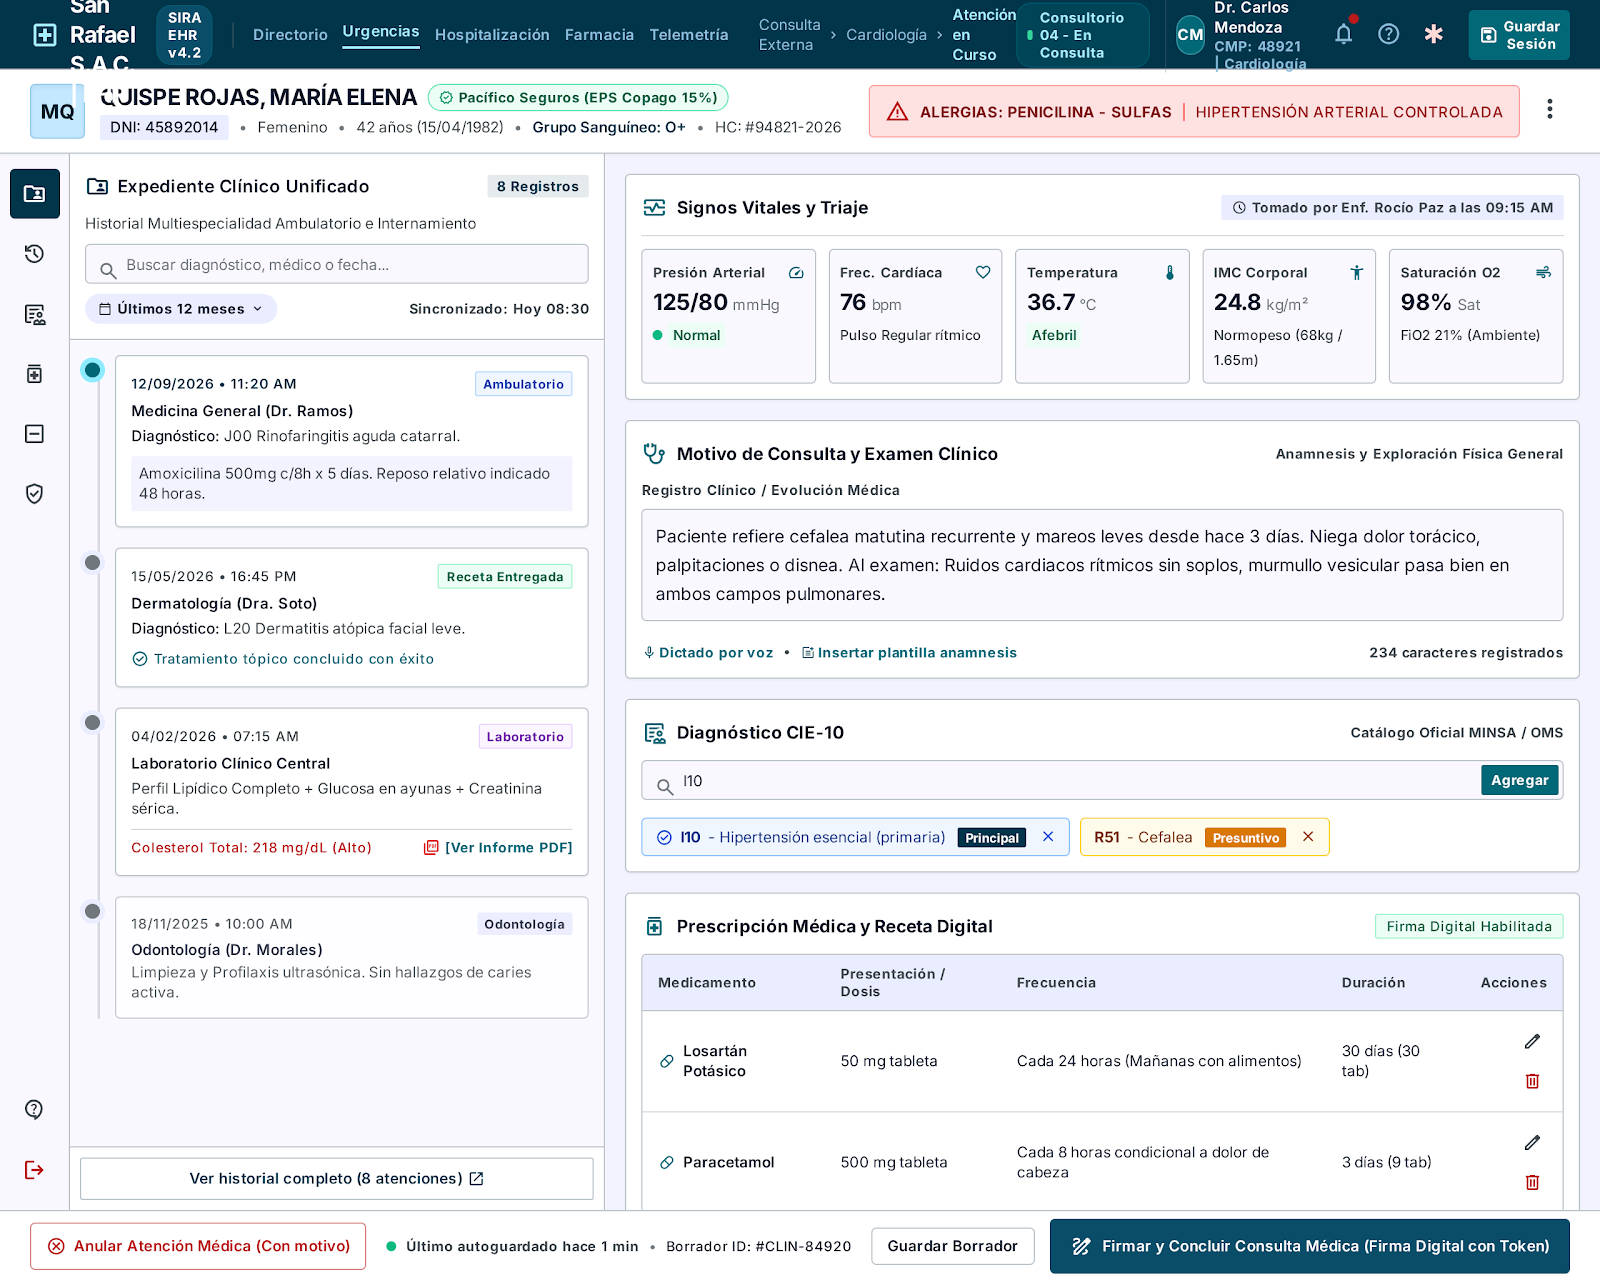
\includegraphics[width=0.95\linewidth]{registroAtencionConsultaHCEunificada.png}
  \caption{Prototipo --- P1. Registro de atención y HCE unificada}
  \label{fig:proto-hce}
\end{figure}

\begin{figure}[!htbp]
  \centering
  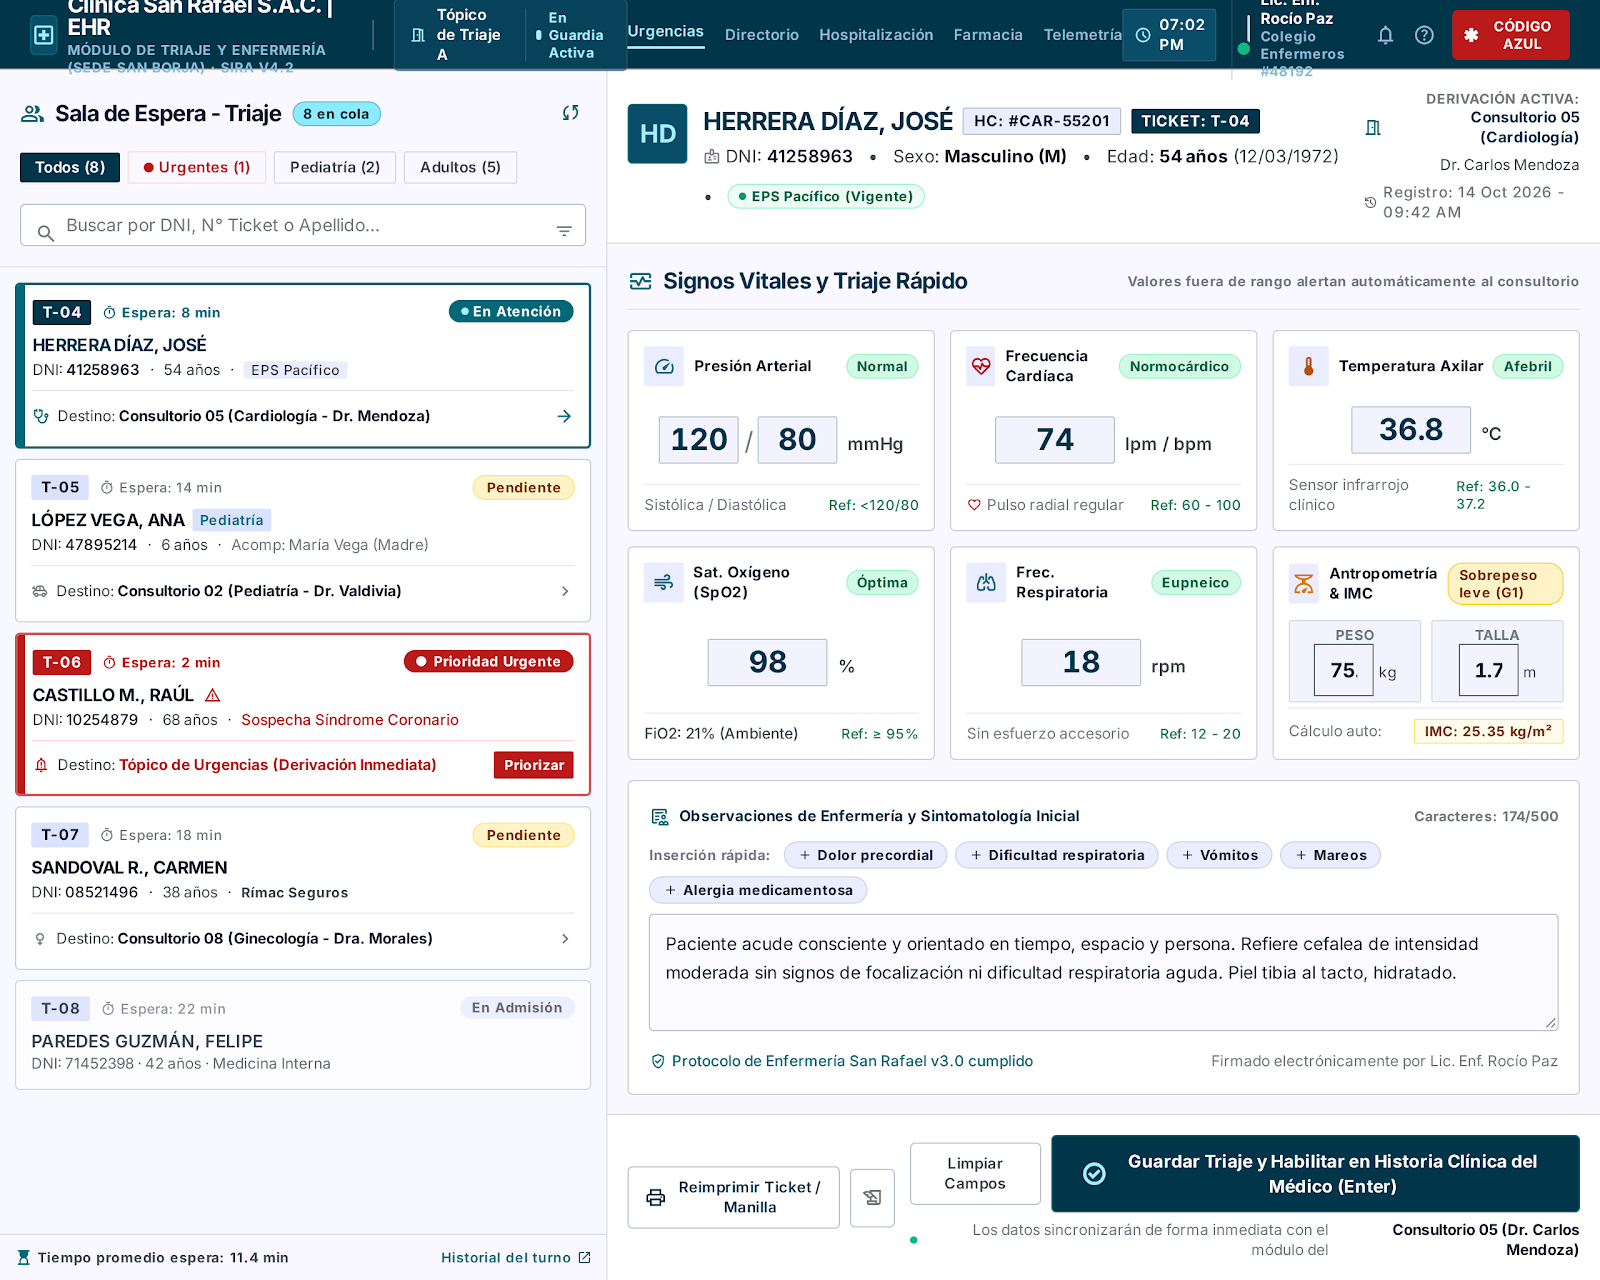
\includegraphics[width=0.95\linewidth]{RegistroTriajeSignosVitales.png}
  \caption{Prototipo --- P3. Registro de triaje y signos vitales}
  \label{fig:proto-triaje}
\end{figure}

\begin{figure}[!htbp]
  \centering
  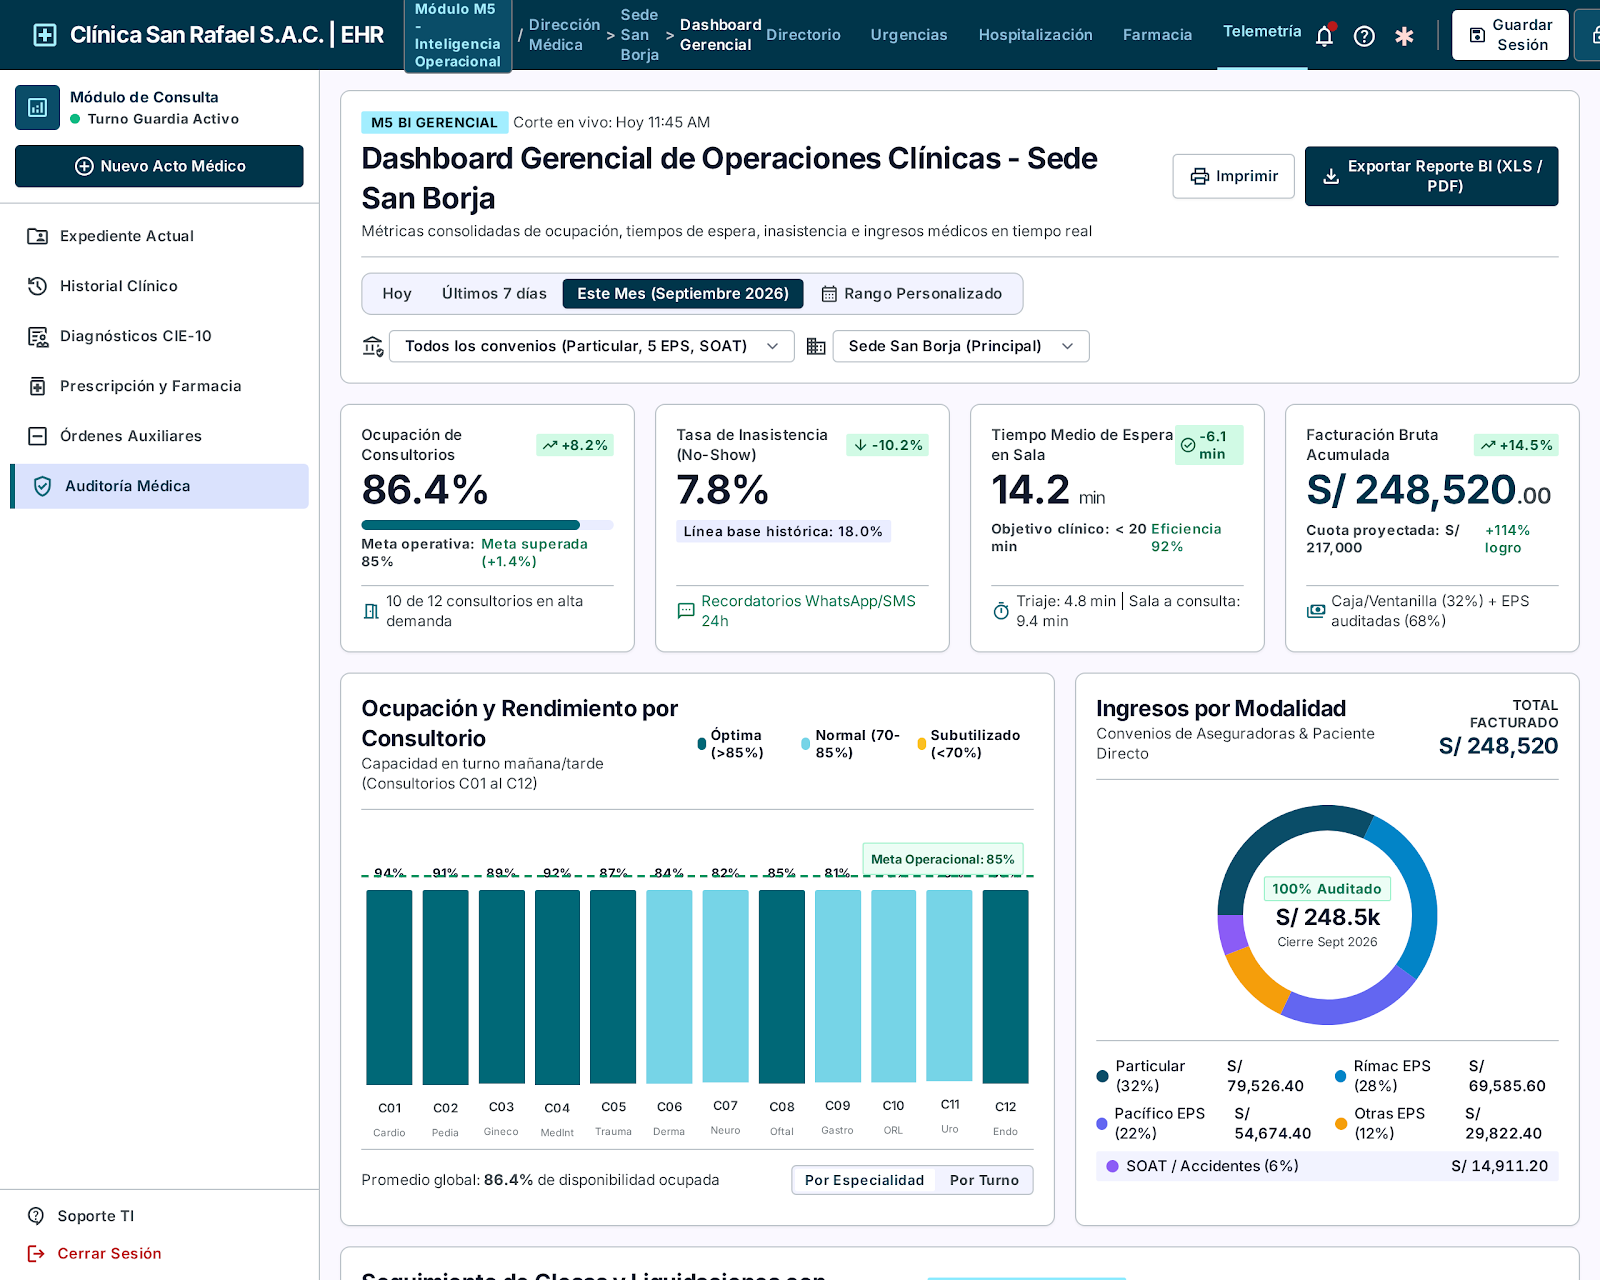
\includegraphics[width=0.95\linewidth]{DashboardGerencial.png}
  \caption{Prototipo --- P4. Tablero gerencial de indicadores}
  \label{fig:proto-dashboard}
\end{figure}

\clearpage
\subsection{Heurísticas de usabilidad aplicadas}

\begin{xltabular}{\linewidth}{|P{5cm}|L|}
  \caption{Heurísticas de Nielsen aplicadas en el prototipo}\label{tab:heuristicas}\\
  \hline
  \rowcolor{guinda}\cab{Heurística (Nielsen)} & \cab{Dónde se aplica en el prototipo} \\ \hline
  \endfirsthead
  \hline
  \rowcolor{guinda}\cab{Heurística (Nielsen)} & \cab{Dónde se aplica en el prototipo} \\ \hline
  \endhead
  Visibilidad del estado del sistema &
    P2: el indicador de 3 pasos marca cuál está completado, activo o pendiente, y cada bloque
    de la matriz muestra si está libre, seleccionado u ocupado. P1: aviso de último autoguardado.
    P3: cada ticket muestra su tiempo de espera y su estado (pendiente, en atención, urgente). \\ \hline
  Prevención de errores &
    P2: los bloques ocupados no se pueden elegir, y la base de datos rechaza igualmente
    cualquier cita superpuesta. P1: la franja de alergias está siempre visible sobre la receta;
    el diagnóstico se elige del catálogo CIE-10; anular exige un motivo. P3: el IMC se calcula
    solo y cada signo vital muestra su rango de referencia. \\ \hline
  Consistencia y estándares &
    Las cuatro pantallas usan la misma barra superior, la misma paleta (rojo solo para alertas
    clínicas) y el botón principal en la esquina inferior derecha; términos del personal de
    salud (CIE-10, triaje, copago, CMP), fechas dd/mm/aaaa y montos en soles. \\ \hline
  Reconocer antes que recordar &
    P1: la cabecera del paciente (documento, edad, convenio, alergias) queda fija mientras el
    médico escribe. P2: el resumen lateral muestra todo lo elegido antes de confirmar.
    P3: botones de inserción rápida para los síntomas frecuentes. \\ \hline
  Ayudar a reconocer y recuperarse de errores &
    P2: ``Cancelar / limpiar selección'' devuelve la matriz a su estado inicial sin perder al
    paciente. P1: ``Guardar borrador'' conserva la atención antes de firmarla; una atención
    firmada se corrige con una anulación que conserva el registro original. \\ \hline
\end{xltabular}

\subsection{Medición del tiempo de la tarea principal}

Procedimiento: un integrante que no diseñó las pantallas realiza la tarea en el prototipo
navegable. El modo de medición del prototipo toma el tiempo desde la pantalla de inicio del rol
hasta la confirmación y lo compara con la meta.

\begin{xltabular}{\linewidth}{|L|P{2.6cm}|P{2cm}|P{2cm}|L|}
  \caption{Medición del tiempo de la tarea principal}\label{tab:tiempo}\\
  \hline
  \rowcolor{guinda}\cab{Tarea principal} & \cab{Participante} & \cab{Meta} & \cab{Tiempo medido} & \cab{Observaciones} \\ \hline
  \endfirsthead
  \hline
  \rowcolor{guinda}\cab{Tarea principal} & \cab{Participante} & \cab{Meta} & \cab{Tiempo medido} & \cab{Observaciones} \\ \hline
  \endhead
  P2: agendar una cita de Pediatría para un paciente ya registrado &
    Rashuaman Sapallanay, Ricco Didier & 3 pasos y $\leq 3$~min & 40.6~s &
    Cumple la meta; completó los 3 pasos hasta emitir el ticket. \\ \hline
  P3: registrar el triaje de un paciente en espera &
    Rashuaman Sapallanay, Ricco Didier & $< 2$~min & 53.0~s &
    Cumple la meta; registró los signos vitales y envió al paciente al consultorio. \\ \hline
\end{xltabular}

% =============================================================================
\newpage
\section{Matriz de trazabilidad}\label{sec:trazabilidad}

Las 14 historias del backlog (ERS, sección 3.7) se rastrean hasta su pantalla
(paso~\ref{sec:prototipo}), su componente (paso~\ref{sec:componentes}) y sus tablas
(paso~\ref{sec:modelo}).

\subsection{\texorpdfstring{Matriz historia $\rightarrow$ pantalla $\rightarrow$ componente $\rightarrow$ tablas}{Matriz historia, pantalla, componente y tablas}}

\begingroup\small
\begin{xltabular}{\linewidth}{|P{2.4cm}|P{2.45cm}|P{2.25cm}|L|L|}
  \caption{Matriz de trazabilidad de historias de usuario}\label{tab:trazabilidad}\\
  \hline
  \rowcolor{guinda}\cab{Historia de usuario} & \cab{Pantalla} & \cab{Componente} & \cab{Tablas} & \cab{Observaciones} \\ \hline
  \endfirsthead
  \hline
  \rowcolor{guinda}\cab{Historia de usuario} & \cab{Pantalla} & \cab{Componente} & \cab{Tablas} & \cab{Observaciones} \\ \hline
  \endhead
  HU01 Consulta de la HCE unificada &
    P1: cabecera del paciente y expediente cronológico & M1, T1, T2 &
    \tb{pacientes}, \tb{atenciones}, \tb{triajes}, \tb{atencion\_diagnosticos},
    \tb{prescripciones}, \tb{resultados}, \tb{bitacora\_auditoria} &
    El acceso de un rol no clínico se rechaza (403) y queda en la bitácora como
    \tb{ACCESO\_DENEGADO}. \\ \hline
  HU02 Agendamiento sin solapamientos &
    P2: pasos 2 y 3 & M2 (M4 para el copago) &
    \tb{citas}, \tb{medicos}, \tb{especialidades}, \tb{consultorios}, \tb{tarifarios\_servicios} &
    Restricciones EXCLUDE por médico y por consultorio (pruebas 1 y 2). \\ \hline
  HU03 Registro y búsqueda del paciente &
    P2: paso 1 & M1, M4 &
    \tb{pacientes}, \tb{convenios} &
    Documento único por tipo y número (prueba 6); el registro de un paciente nuevo se abre
    desde el paso 1. \\ \hline
  HU04 Atención con CIE-10 y receta &
    P1: diagnóstico, receta y ``Firmar y finalizar'' & M1 &
    \tb{atenciones}, \tb{atencion\_diagnosticos}, \tb{diagnosticos\_cie10}, \tb{prescripciones} &
    Un solo diagnóstico principal por atención (prueba 7). \\ \hline
  HU05 Triaje y signos vitales &
    P3 & M1 (M2 para el check-in) &
    \tb{triajes}, \tb{atenciones}, \tb{citas} &
    Rangos de signos vitales validados en la base (prueba 10). \\ \hline
  HU06 Reprogramación y cancelación &
    P2: matriz de horarios sobre una cita existente & M2, T3 &
    \tb{citas}, \tb{outbox\_notificaciones} &
    \tb{id\_cita\_origen} enlaza la cita nueva con la anterior; el motivo es obligatorio
    (\tb{chk\_cita\_motivo}). \\ \hline
  HU07 Recordatorio a 24~h &
    P2: interruptor del paso 3 & T3, M2 &
    \tb{outbox\_notificaciones}, \tb{citas} &
    El envío lo hace un proceso en segundo plano. \\ \hline
  HU08 Anulación lógica &
    P1: ``Anular atención (con motivo)'' & M1, T2 &
    \tb{atenciones}, \tb{bitacora\_auditoria} &
    Sin DELETE (prueba 3); motivo de al menos 20 caracteres (prueba 4). \\ \hline
  HU09 Órdenes de examen &
    P1: ``Emitir orden de examen'' & M3 (M4 catálogo) &
    \tb{ordenes\_examen}, \tb{servicios\_medicos} &
    La bandeja del laboratorio se diseña en el Sprint~2. \\ \hline
  HU10 Resultados en $\leq 4$~h &
    P1: tarjeta de laboratorio con ``Ver informe PDF'' & M3, T3 &
    \tb{resultados}, \tb{ordenes\_examen}, \tb{outbox\_notificaciones} &
    \tb{fecha\_resultado} $\geq$ \tb{fecha\_toma\_muestra}; la carga del resultado se diseña en el
    Sprint~2. \\ \hline
  HU11 Facturación por convenio &
    P2, paso 3: copago estimado & M4 &
    \tb{facturas}, \tb{factura\_detalle}, \tb{tarifarios\_servicios}, \tb{convenios},
    \tb{servicios\_medicos} &
    Montos cuadrados por línea (prueba 8) y vigencias sin superponer (prueba 9). \\ \hline
  HU12 Seguimiento de glosas &
    P4: tabla de glosas & M4, T2 &
    \tb{glosas}, \tb{facturas} &
    El registro de una glosa nueva se diseña en el Sprint~2. \\ \hline
  HU13 Tablero gerencial &
    P4 & M5 &
    Solo lectura: \tb{citas}, \tb{consultorios}, \tb{especialidades}, \tb{atenciones},
    \tb{factura\_detalle}, \tb{glosas}, \tb{convenios} &
    No muestra datos clínicos de pacientes. \\ \hline
  HU14 Portal del paciente &
    Sin pantalla (módulo condicional, RN-06) & M6 $\rightarrow$ M2, T1 &
    \tb{citas} (canal PORTAL\_WEB), \tb{pacientes}, \tb{outbox\_notificaciones} &
    Reutiliza las reglas de agenda de M2. \\ \hline
\end{xltabular}
\endgroup

\subsection{Verificación inversa: de las tablas a las historias}

Las 22 tablas tienen al menos una historia que las justifica; \tb{usuarios} y \tb{roles}
responden al RNF-002, común a todas las historias.

\begingroup\small
\begin{xltabular}{\linewidth}{|P{4cm}|L|L|}
  \caption{Historias de usuario que justifican cada tabla}\label{tab:inversa}\\
  \hline
  \rowcolor{guinda}\cab{Tabla} & \cab{Historias de usuario que la justifican} & \cab{Observaciones} \\ \hline
  \endfirsthead
  \hline
  \rowcolor{guinda}\cab{Tabla} & \cab{Historias de usuario que la justifican} & \cab{Observaciones} \\ \hline
  \endhead
  \tb{pacientes} & HU01, HU03 (y HU02, HU14 al agendar) & M1 \\ \hline
  \tb{atenciones} & HU01, HU04, HU08 & M1; anulación lógica \\ \hline
  \tb{triajes} & HU05 & M1; una por atención \\ \hline
  \tb{diagnosticos\_cie10} & HU04 & M1; catálogo \\ \hline
  \tb{atencion\_diagnosticos} & HU04, HU01 & M1 \\ \hline
  \tb{prescripciones} & HU04, HU01 & M1 \\ \hline
  \tb{citas} & HU02, HU06, HU05 (check-in), HU14 & M2 \\ \hline
  \tb{medicos} & HU02, HU04 & M2 \\ \hline
  \tb{especialidades} & HU02, HU13 & M2; catálogo \\ \hline
  \tb{consultorios} & HU02, HU13 & M2; los 12 consultorios \\ \hline
  \tb{ordenes\_examen} & HU09, HU10 & M3 \\ \hline
  \tb{resultados} & HU10, HU01 & M3 \\ \hline
  \tb{convenios} & HU03, HU11 & M4; catálogo \\ \hline
  \tb{servicios\_medicos} & HU09, HU11 & M4; catálogo \\ \hline
  \tb{tarifarios\_servicios} & HU11 (y HU02 para el copago estimado) & M4 \\ \hline
  \tb{facturas} & HU11, HU12 & M4 \\ \hline
  \tb{factura\_detalle} & HU11, HU13 & M4 \\ \hline
  \tb{glosas} & HU12, HU13 & M4 \\ \hline
  \tb{outbox\_notificaciones} & HU07, HU06, HU10 & T3 \\ \hline
  \tb{bitacora\_auditoria} & HU08, HU01 (escenario 2) & T2; inmutable \\ \hline
  \tb{usuarios} & Todas (RNF-002); HU01 escenario 2 & T1 \\ \hline
  \tb{roles} & Todas (RNF-002); HU01 escenario 2 & T1 \\ \hline
\end{xltabular}
\endgroup

% =============================================================================
\newpage
\section*{Anexo A. Declaración de uso de herramientas de IA y de terceros}
\addcontentsline{toc}{section}{Anexo A. Declaración de uso de herramientas de IA y de terceros}

Conforme a la disposición de integridad académica del proyecto integrador, el equipo declara
las herramientas de inteligencia artificial o de terceros utilizadas en este entregable. Todo
el contenido declarado fue revisado por el equipo, que puede explicarlo.

\begin{xltabular}{\linewidth}{|P{3.1cm}|L|P{2.4cm}|P{3.7cm}|}
  \caption{Herramientas de IA y de terceros utilizadas}\label{tab:declaracion-ia}\\
  \hline
  \rowcolor{guinda}\cab{Herramienta} & \cab{Uso que se le dio} & \cab{Parte del entregable} & \cab{Revisado por} \\ \hline
  \endfirsthead
  \hline
  \rowcolor{guinda}\cab{Herramienta} & \cab{Uso que se le dio} & \cab{Parte del entregable} & \cab{Revisado por} \\ \hline
  \endhead
  Claude (Anthropic) & Redacción de las decisiones tomadas por el equipo en los pasos 1 a 5;
    apoyo en los scripts SQL, los datos de prueba, el código de los diagramas y las indicaciones
    del prototipo navegable, que el equipo ejecutó y verificó & Pasos 1 a 5 &
    Rashuaman Sapallanay, Ricco Didier \newline Albino Soto, Christopher Henrry \newline
    Inga Champi, Franz Joe \\ \hline
  Google Stitch & Pantallas de alta fidelidad a partir de la especificación de pantallas del
    equipo & Paso 4 (figuras del prototipo) & Albino Soto, Christopher Henrry \\ \hline
  Figma Make & Prototipo navegable a partir de las pantallas del equipo, con el modo de medición
    del tiempo de las tareas & Paso 4 (prototipo navegable y medición) &
    Rashuaman Sapallanay, Ricco Didier \\ \hline
  Mermaid Live Editor & Exportación del diagrama de componentes y del modelo entidad-relación
    desde su código fuente & Pasos 1 y 2 & Inga Champi, Franz Joe; Rashuaman Sapallanay, Ricco Didier \\ \hline
\end{xltabular}

\end{document}
